\chapter{High-intensity photoassociation spectroscopy of a halo molecule} \label{ch:chap4}
\section{Probing the ground state potential} \label{sec:highE_intro}
In this chapter we study the least-bound vibrational level of the X$^1\Sigma_g^+$ electronic ground state of the $^{86}$Sr$_2$ dimer in a high-intensity regime.
Previous studies of the molecular states of the X$^1\Sigma_g^+$ ground state potential have been performed using strontium-88, due to its high natural abundance, and strontium-84, because of it's amenable scattering properties. \cite{Reinaudi2012, McGuyer2014, McGuyer2015a, rom12, Stellmer2012}.

This work presents the first two-photon photoassociation study of the ground state of $^{86}$Sr.
All previous PA experiments with this isotope have been one-photon photoassociation to excited electronic states \cite{Mickelson2005,Borkowski2014a,Reschovsky2018}.
The large $s$-wave scattering length, $\sim$800\,a$_0$, for this isotope is indicative of a near-threshold bound state known as a halo molecule.
Direct photoassociation to this halo state revealed several unanticipated phenomena discussed in this chapter including AC Stark shifts comparable to the halo molecule binding energy and multi-photon resonance processes \cite{Kon2018}.

This work is expanded upon in Ch.\,\ref{ch:chap5} with a low-intensity study that precisely determined the halo binding energy and using this measurement, improves upon the previous best determinations of the scattering lengths of all strontium isotopes via mass-scaling.
In these initial experiments, we explore some of the novel effects of photoassociation to a halo state with a focus on understanding the AC Stark shifts and developing a useful theoretical framework for describing this unique photoassociation regime.

As discussed in previous chapters, two-photon PAS can be used to directly populate molecular levels and may be described with the formalism of Bohn and Julienne \cite{Bohn1999}.
However, this approach assumes the two driving lasers are of sufficiently different frequencies that each independently drives a specific transition, as in the typical $\Lambda$-model \cite{Wynar2000, Bohn1996}.
In the regime of PAS to a halo state, the laser frequencies differ by only up to $\sim\!300$\,kHz, much smaller than the typical intermediate state detuning of several MHz.
Thus, both lasers must be considered to act on each leg of the transition simultaneously.
The effects of this two-frequency coupling were explored through a collaboration with the theory group of Kaden Hazzard to develop simple models that are able to reproduce the key experimental observations and features.

In the following, we present the experimental results of high-intensity PAS to the halo state and develop lineshape models based on the theory of Bohn and Julienne to extract the halo state binding energy.
Next, we'll compare our experimental data to numerical simulations of a three-level model.
This model subsequently becomes the basis of a Floquet treatment which results in an analytic form for describing and predicting AC Stark shifts of the halo state.
This is used to consider the observed frequency dependence of the halo state energy and estimate the bound-bound coupling strength between the intermediate and halo states.

\section{Experimental setup} \label{sec:highE_methods}
	\begin{figure} 
	\centerline{
	  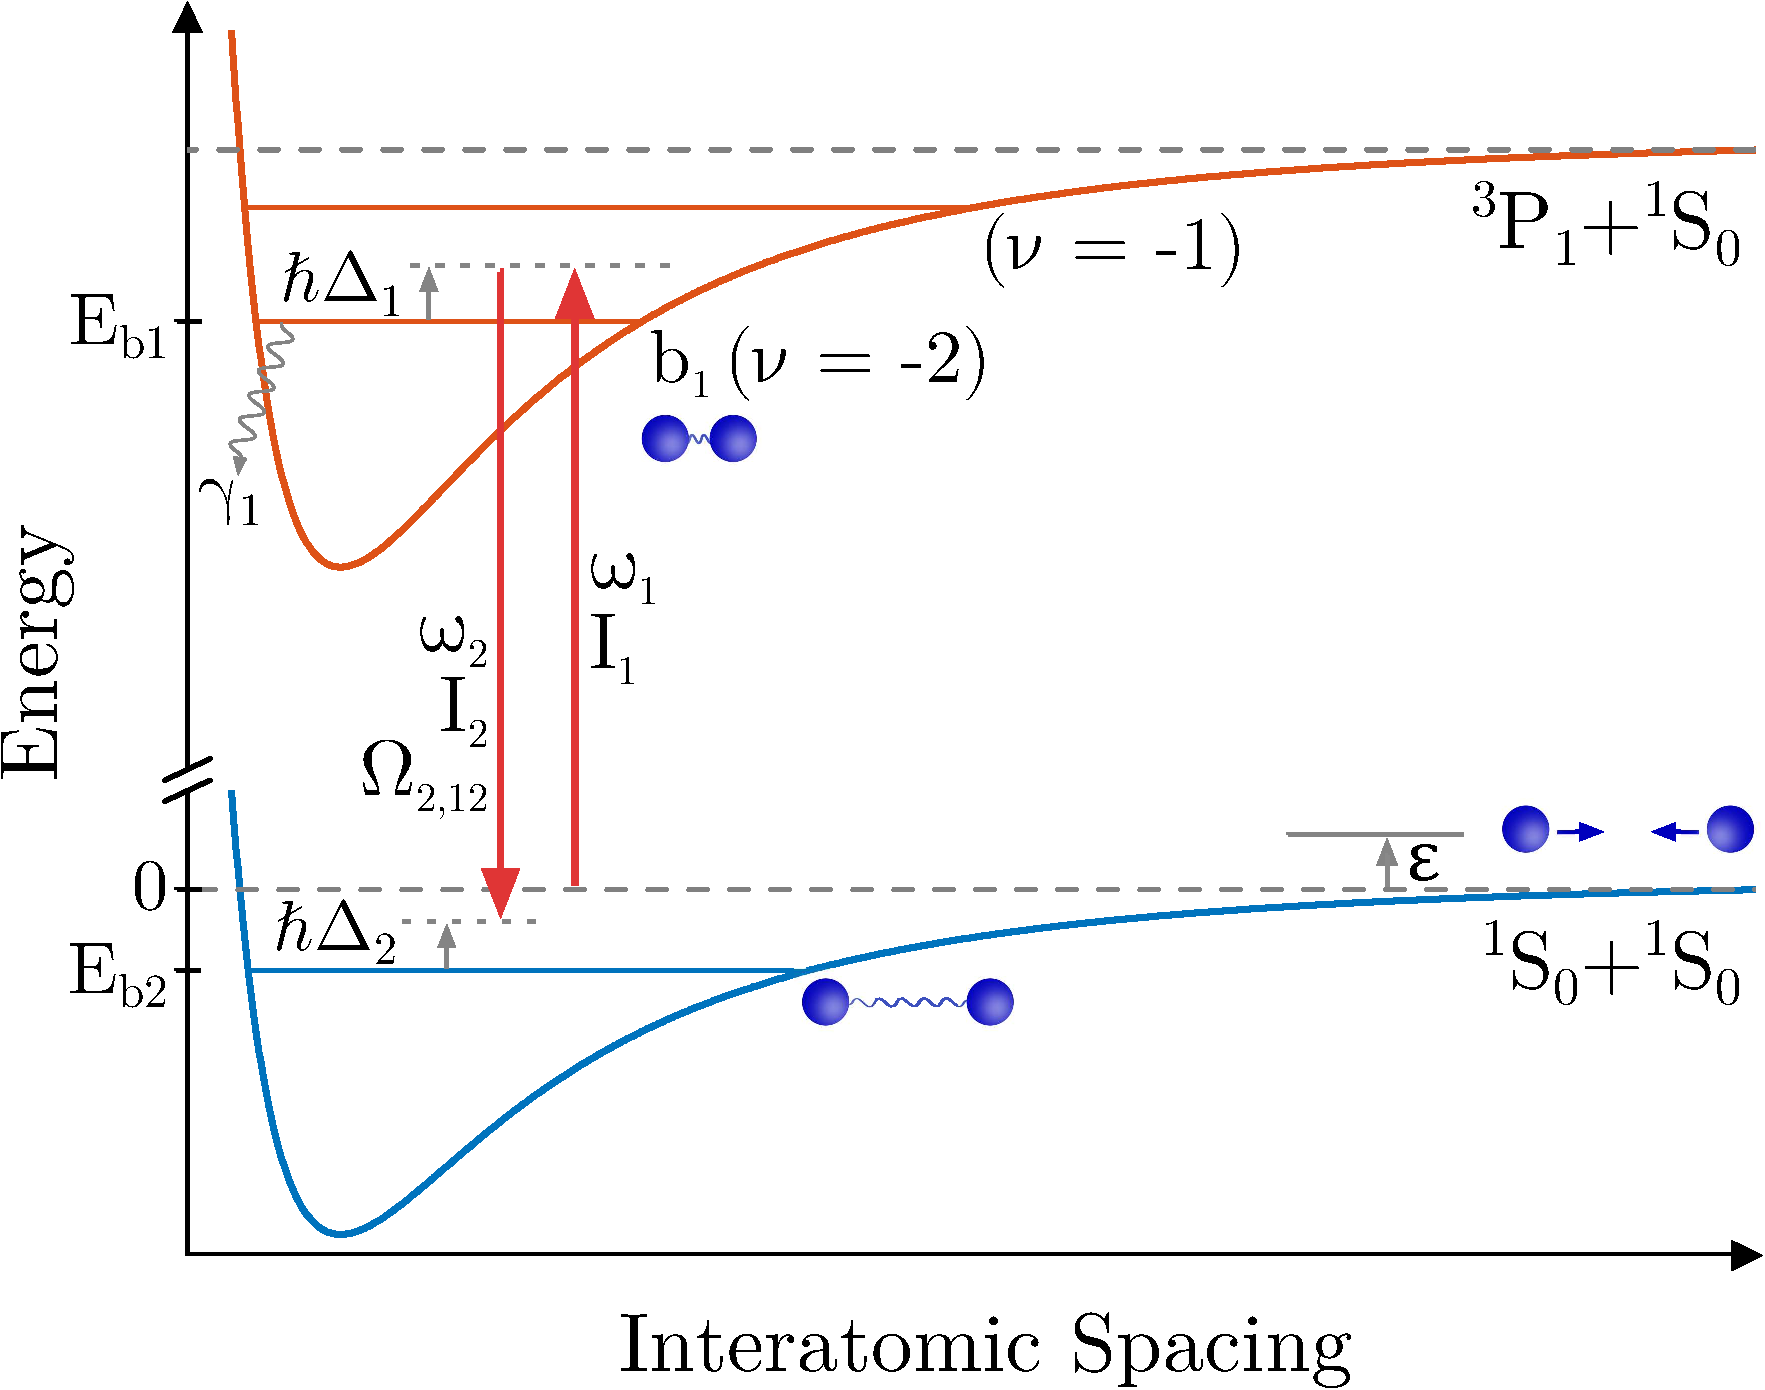
\includegraphics[width=\textwidth]{sr_pa_potential.pdf}}
	  \caption{$^{86}$Sr$_2$ halo molecule excitation scheme}{Two-photon photoassociation diagram. The energy of two well-separated $^1S_0$ atoms at rest is taken as zero. $\epsilon$ is the kinetic energy of the colliding atom pair. $E_{b1}$ is the unperturbed energy of the bound state of the excited molecular potential that is near resonance with the free-bound laser, which in these experiments is the second-least-bound level of the excited molecular potential $\nu=-2$. $E_{b2}$ ($<0$) is the energy of the least-bound state of the ground molecular potential. The photon of energy $\hbar \omega_1$ is detuned from $E_{b1}$ by $\hbar \Delta_1$ for $\epsilon=0$, while the two-photon detuning from $E_{b2}$ is $\hbar \Delta_2$. The decay rate of $b_1$ is $\gamma_1$. Stark and collisional frequency shifts are neglected in this schematic.}
	  \label{fig:PASDiagram}
	\end{figure}
Fig.\,\ref{fig:PASDiagram} shows the excitation scheme used to probe the halo state in $^{86}$Sr using two-photon Raman photoassociation \cite{Jones2006}, in which two laser fields couple colliding atoms to the least-bound state of the ground molecular potential. 
%The sample temperature is low enough that collisions are entirely $s$-wave. 
$^{86}$Sr has no nuclear spin and a $^1S_0$ electronic ground state, leading to a single X$^1\Sigma_g^+$ ground electronic molecular potential.
The target state for the two-photon transition has total angular momentum $J=0$ and halo state energy $E_{b2}(<0)$, which we label as $b_2$.
The dominant intermediate state, $b_1$, with energy E$_{b1}$, is the $J=1$ rotational state of the second least-bound $\nu=-2$ vibrational level on the $0^+_u$ molecular potential, which asymptotically connects to the $^1S_0\,+\,^3P_1$ asymptote at long range \cite{MartinezDeEscobar2008}.
This state is bound by $44.246(10)$\,MHz \cite{Borkowski2014a, Reschovsky2018}.
We define $\Delta_1=\omega_1-\text{E}_{b1}/\hbar$ and $\Delta_2=\omega_1-\omega_2-\text{E}_{b2}/\hbar$ as the one-photon detuning from state $b_1$ and two-photon detuning from state $b_2$ respectively for an initial scattering state with collision energy $\epsilon=0$.
The Rabi frequency, $\Omega_{2,12}$, characterizes coupling between states $b_1$ and $b_2$ due to the laser field at $\omega_2$ with single-beam intensity $I_2$.
Because the binding energy of the halo molecule is very small compared to $\Delta_1$, both laser frequencies are near resonance with the $\nu=-2$ state. 
The least-bound $\nu=-1$, $J=1$ excited molecular state, bound by $1.633(1)$\,MHz, and the excited atomic state lie near enough in energy to the $\nu = -2$ state that they can also effect our observations.	

The small detuning between $\omega_1$ and $\omega_2$ results in an atypical consideration of the accessible resonance conditions during the Raman process.
Fig.\,\ref{fig:haloResProcess}a shows the two scenarios which lead to resonance with the halo state when $\omega_1$ is held fixed and $\omega_2$ is varied.
	\begin{figure} 
	\centerline{
	  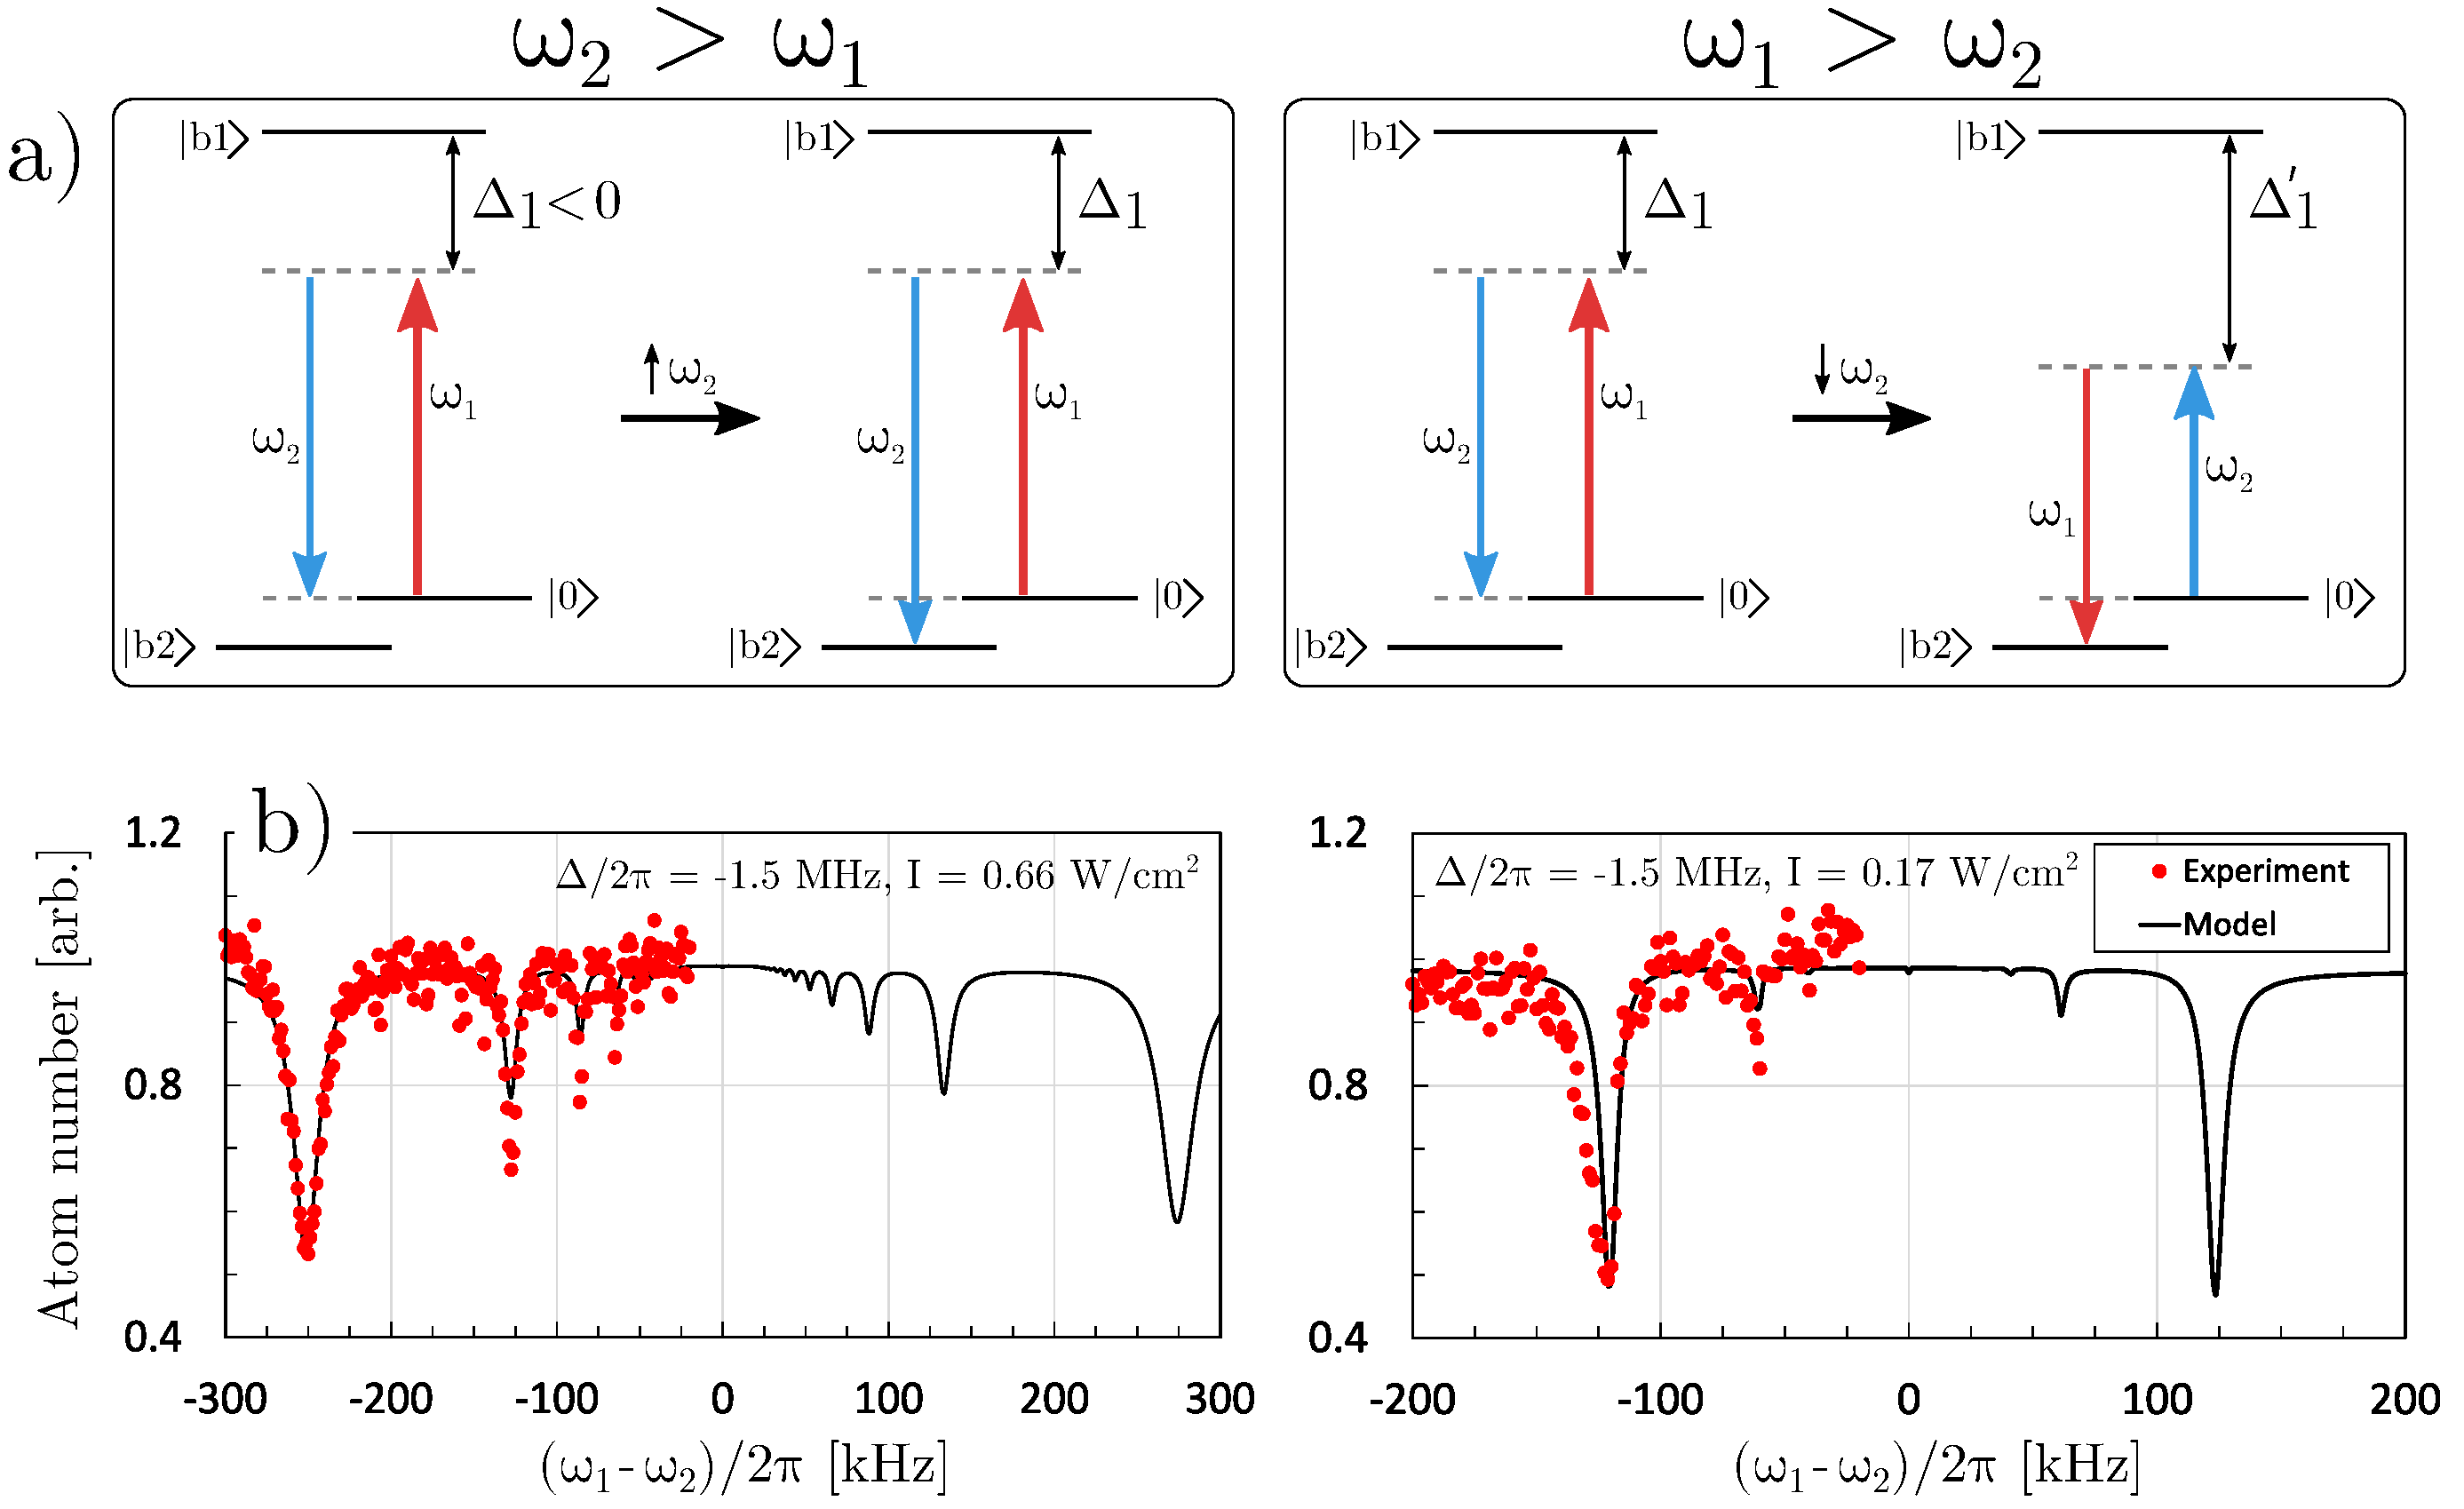
\includegraphics[width=\textwidth]{excitationScheme.pdf}}
	  \caption{Accessible halo resonance PAS processes}{Effects of fixing $\omega_1$ and varying $\omega_2$. Consider the state \ket{b2} to be fixed. a) The left and right panels illustrate scanning $\omega_2$ relative to $\omega_1$. Within each panel, the lasers start with $\omega_1 = \omega_2$ and $\Delta_2 = -E_b/\hbar$. Scanning $\omega_2$ will fulfill the resonance condition in both scenarios but also lead to a change in $\Delta_1$ if $\omega_1 > \omega_2$.  b) Example simulated spectra compared with experimental PAS. The development of the model is described in Sec.\,\ref{sec:highE_theory}. For both simulations, the "positive" axis is the configuration where $\omega_2 \geq \omega_1$ and the negative axis is the opposite. Note the asymmetry in the resonance frequency for $I=0.66$\,W/cm$^2$.}
	  \label{fig:haloResProcess}
	\end{figure}
The left panel, when $\omega_2 \geq \omega_1$, shows $\Delta_1$ remains fixed while scanning the two-photon energy.
This holds constant the bound-bound coupling between the halo and intermediate state.
In the opposite case, when $\omega_2 \leq \omega_1$, the halo resonance condition can still be satisfied as $\omega_2$ is varied, though at the expense of also varying $\Delta_1$.
This behavior is equivalent to fixing $\omega_2$ and scanning $\omega_1$ in a typical $\Lambda$-type Raman scheme, but warrants our attention because of the interchangeability of the excitation lasers.

The latter configuration, which couples $\omega_2$ and $\Delta_1$, was used during our photoassociation experiments.
The effects on the observable spectra between these two schemes was considered using a three-level model, Sec.\,\ref{sec:highE_theory}, to evaluate both scenarios of laser detuning across the complete range of our data.
Fig.\,\ref{fig:haloResProcess}b shows two simulated spectra in the regime of strongest coupling accessible by our experiments.
The higher intensity spectrum, $I=0.66$\,W/cm$^2$, shows that coupling between $\Delta_1$ and $\omega_2$ can noticeably shift the resonance energy of the halo state. 
Importantly, this prediction is in a regime where E$_{b2} \sim \Delta_1$, which applies to only a small subset of our measurements.
Most of our data is in a regime where $\Delta_2 \ll \Delta_1$ thus we neglect variation of the AC Stark shift with $\omega_2$.

%Future work focused on high precision photoassociation of the $*{86}$Sr halo state may capitalize on this asymmetry as a test of a model's predictive ability or to ensure symmetry of the probe lasers in a regime where the change in AC Stark shift is vanishingly small.
 % by $\approx$10\% between configurations.
%% Sample properties and trap description

Spectroscopy is performed in a crossed beam optical dipole trap generated from a $1064$\,nm laser propagating perpendicular to gravity with spot sizes at the atoms of $300\,\mu\text{m}\,\times\,60\,\mu\text{m}$ and $400\,\mu\text{m}\,\times\,40\,\mu\text{m}$, with both short axes parallel to gravity.
Further details are available in Sec.\,\ref{ssec:1064sys}.
Typical atom numbers are several hundred thousand and sample temperatures of approximately $300\,\text{nK}$.
Peak densities are between \peakDens{1 - 2}{12}.
Following forced evaporative cooling, the atoms are allowed to thermally equilibrate before being illuminated by the photoassociation lasers for $\approx\!1 - 10$ milliseconds.
The number of remaining ground-state atoms and the sample temperature are measured using absorption imaging after release from the trap and subsequent expansion during time-of-flight.
Trap oscillation frequencies are determined by measuring dipole and breathing collective mode frequencies, which allow determination of trap volume and sample density.

%% PAS light generations
We generate the two photons for spectroscopy as shown in Fig.\,\ref{fig:pas_light_gen}.
	\begin{figure} 
		\centerline{
		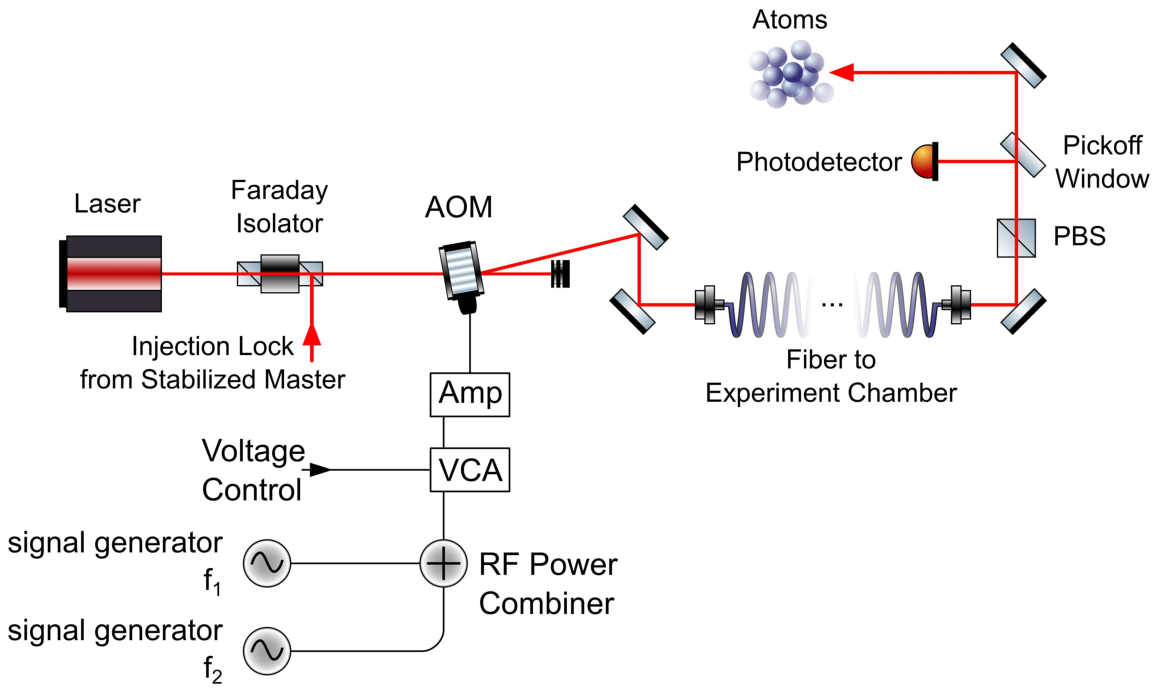
\includegraphics[width=\textwidth]{pa_exp_setup.pdf}}
		\caption{Schematic of PAS light generation}{Light for these experiments is generated by the spectroscopy slave laser setup discussed in Sec.\,\ref{sec:specSlave}. Light at two controllable frequencies is generated with a single acousto-optic modulator (AOM) and delivered to the atoms with an optical fiber. The beat note between the two frequencies is monitored after the fiber.}
		\label{fig:pas_light_gen}
	\end{figure} 
Using an AOM, these photons are derived from the output of a slave diode laser that is injection locked from the master $689\,\text{nm}$ laser.
Two precisely controlled RF frequencies are applied to a single AOM to generate both beams.
These frequencies are separated by less than $300\,\text{kHz}$, and the diffracted beams corresponding to each frequency component are unresolvd and appear as a single beam that is coupled into a single-mode, polarization-maintaining optical fiber.

This fiber output is launched near the science chamber and shaped with output optics that yield a 450\,$\mu$m spherical waist at the atoms, much larger than the size of the atom cloud.
The light from this fiber is linearly polarized such that the polarization vector is parallel to gravity.
The optical fiber ensures that the wavevector of the two photons will be parallel.
This allows us to neglect any effects of Doppler broadening that might result from photoassociation near an intercombination line.

By using a single laser source and applying both frequencies to a single acousto-optic modulator, we establish phase coherence and RF precision frequency differences between the $\omega_1$ and $\omega_2$ photons.
Reduction of the beat note contrast is the primary limiting factor of the accessible range of $\Delta_2$ for this spectroscopy setup.
This is due to misalignment into the optical fiber resulting from the varying angular deviation out of the AOM as the RF frequency difference is increased.
We partially compensate for this misalignment by increasing the RF amplitude of one drive frequency to maintain high beat note contrast.
WHowever, we observe significant reduction in contrast, which we were unable to compensate for, when the two drive frequencies differ by more than $\approx\!300\,\text{kHz}$. 

During the course of our experiments we found that mild environmental perturbations resulted in slow variation (on the order of 1\,s) of the light intensity through the optical fiber.
Such amplitude modulations are not uncommon in laser systems and are typically compensated by using a closed-loop intensity stabilization circuit. 
%However, after construction of such a power lock the compoenets did not react quickly enough and there was a significant overshoot which resulted in an uncontrolled amount of light illuminating the atoms during short exposures. 
However, this circuit was inadequate for short-time exposures due to the acquisition process being long compared to our desired pulse width.
This led us to implement the digital based infinite sample and hold mechanism for reduced intensity variability described in Sec.\,\ref{sec:infSH}. 
The sample and hold system provided increased intensity stability with a 5\% standard deviation during a typical experiment. 
The beat signal of the two light fields after the fiber was monitored on a photodiode and the RF powers adjusted to ensure matched intensities for the two frequency components ($I_1 = I_2 \equiv I$).
Fig.\,\ref{fig:PASbeamStability} shows a typical histogram of the recorded intensities during an experimental scan along with a sample beat note showing the contrast.
	\begin{figure}
		\centerline{
		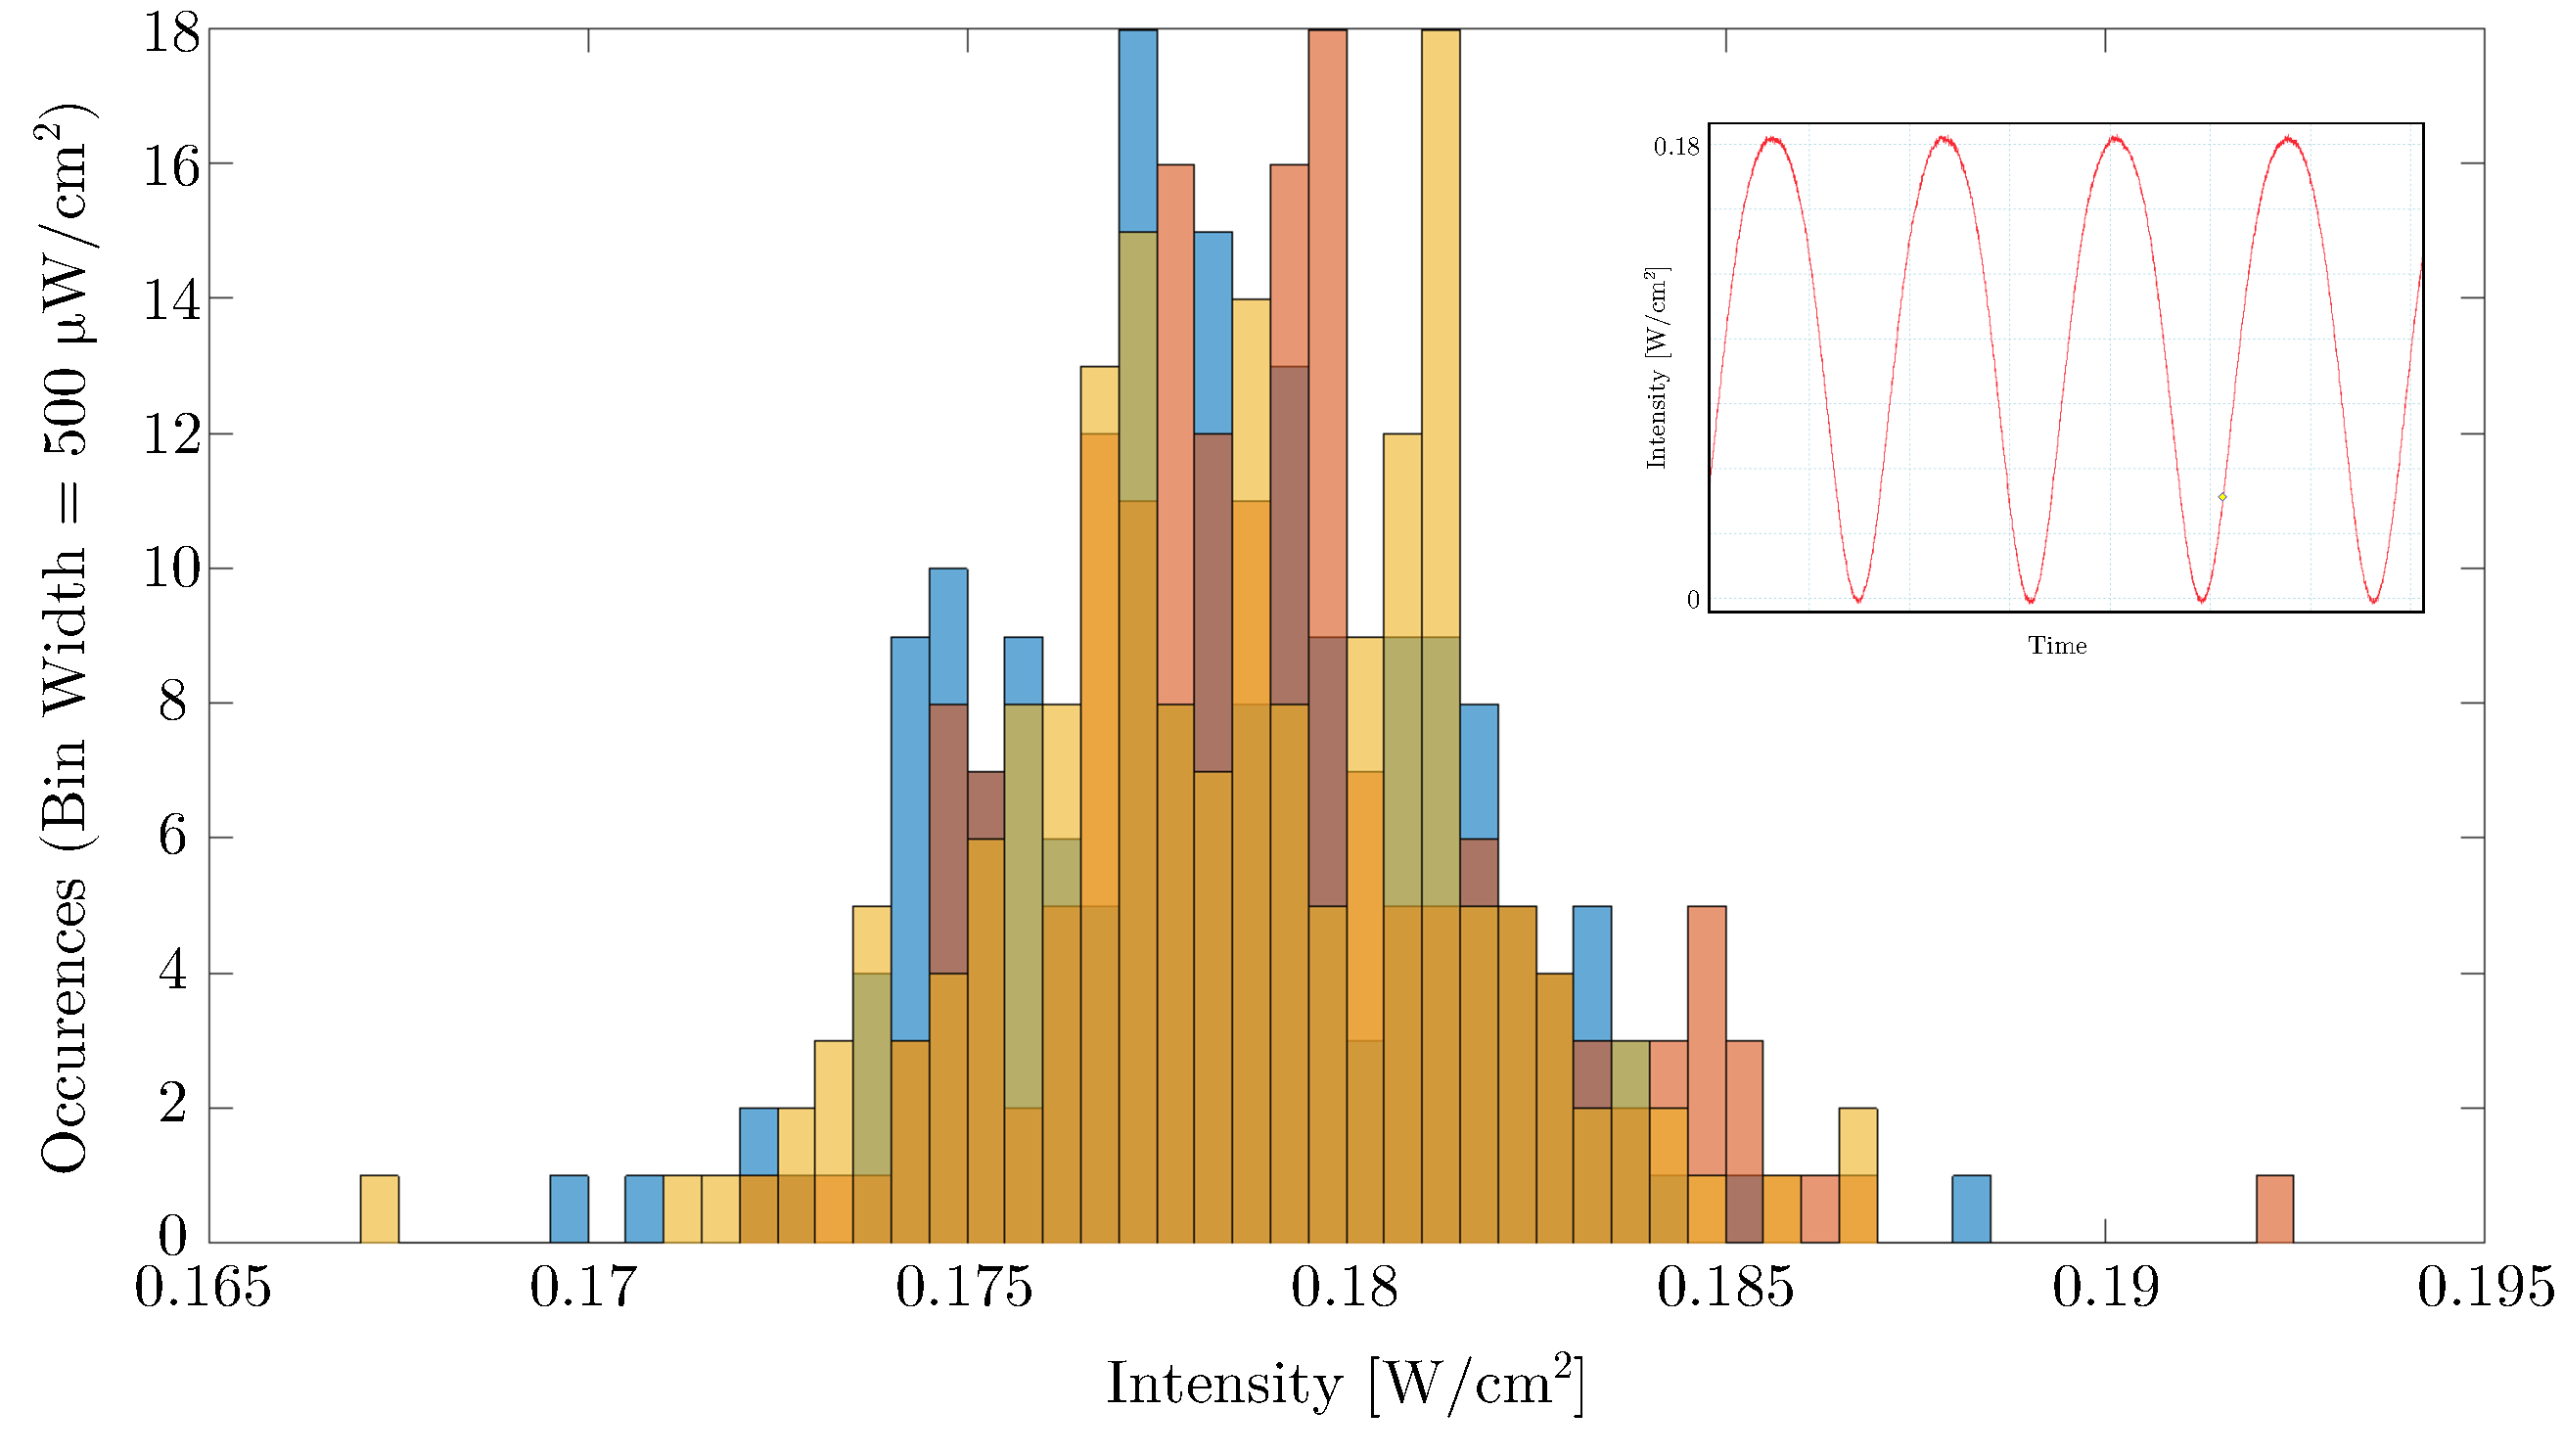
\includegraphics[width=\textwidth]{pasBeamCharacter.pdf}}
		\caption{Histogram of PAS beam intensity variation}{Sample intensity variation during a set of photoassociation scans. Different colors denote multiple scans separated in time which are averaged. The inset shows a sample beat note and typical contrast.}
		\label{fig:PASbeamStability}
	\end{figure} 

%
%As described in \hl{some section} the slave laser is frequency stabiliezed at +42 MHz of the 86Sr $\gs\,\rightarrow\,\ex$ atomic transition. The AOM then shifts the light the remaining $\approx$ 86 MHz to set the detuning around the $\nu=-2$ bound state of the \intPot{\gs}{\ex} potential. 
%Setting of $\Delta_1$ is done by removing one of the frequencies, peaking up the diffraction angle and alignment into the fiber. 

%Regarding the general process 
%
%Using the \intPot{\gs}{\ex} interatomic potential, we perform a raman process using the $\nu=-2$ bound state which has a binding energy of E$_b=-44 \text{MHz}$ \hl{cite improved binding en}. Sample pre 
%
%We used strontium 86 in a thermal gas at temperatures between 30 and 1000 nK. Typical peak densitieis were around $\peakDens{1}{12}$. 
%
%Raman process using the second bound state of the \intPot{\gs}{\ex} interatomic potential
%
%After the atoms have equilibrated in the final ODT configuration, the PA lasers are applied (Fig.\ \ref{PASDiagram}). A single acousto-optic modulator, driven with two RF frequencies, is used to generate both PA beams. Light is derived from a frequency-stablized master laser (Fig.\ \ref{Experimental Setup}) and coupled into a single-mode optical fiber 

%$I_{689}$ is varied to obtain the intensity-dependence of the two-photon transition.

%(One could in principle vary the power of both light fields independently and measure how the two-photon line position changes. This will allow us to decouple the contributing factors to the AC Stark shift. If we are going to develop a theory of the multiphoton line, it will have to be able to treat this regime as well. )



\section{Modeling the photoassociative loss} \label{sec:highE_paLoss}
%due to radiative decay from the intermediate, excited electronic state, and from collisions between molecules and background atoms.
We observe the effects of photoassociation as a loss of atoms from the optical dipole trap as a function of the frequency difference, $\Delta_2$, between the two excitation lasers.
Fig.\,\ref{fig:highIntSpectra} shows several spectra resulting from photoassociation to the $^{86}$Sr$_2$ halo state as the excitation beam intensity is varied.
Intensities are specified by the single-beam intensities, $I$ as defined in the previous section, with the average total near-resonant intensity illuminating the atoms given by $I_{\text{689}}=2I$.
In each of the spectra, the characteristic asymmetric tail of a photoassociation process sensitive to the relative collision energy distribution of the trapped atoms can be observed.
Each spectra are averaged over several scans and the error bars give the standard error calculated for each detuning $\Delta_2$.
	\begin{figure}
		\centerline{
		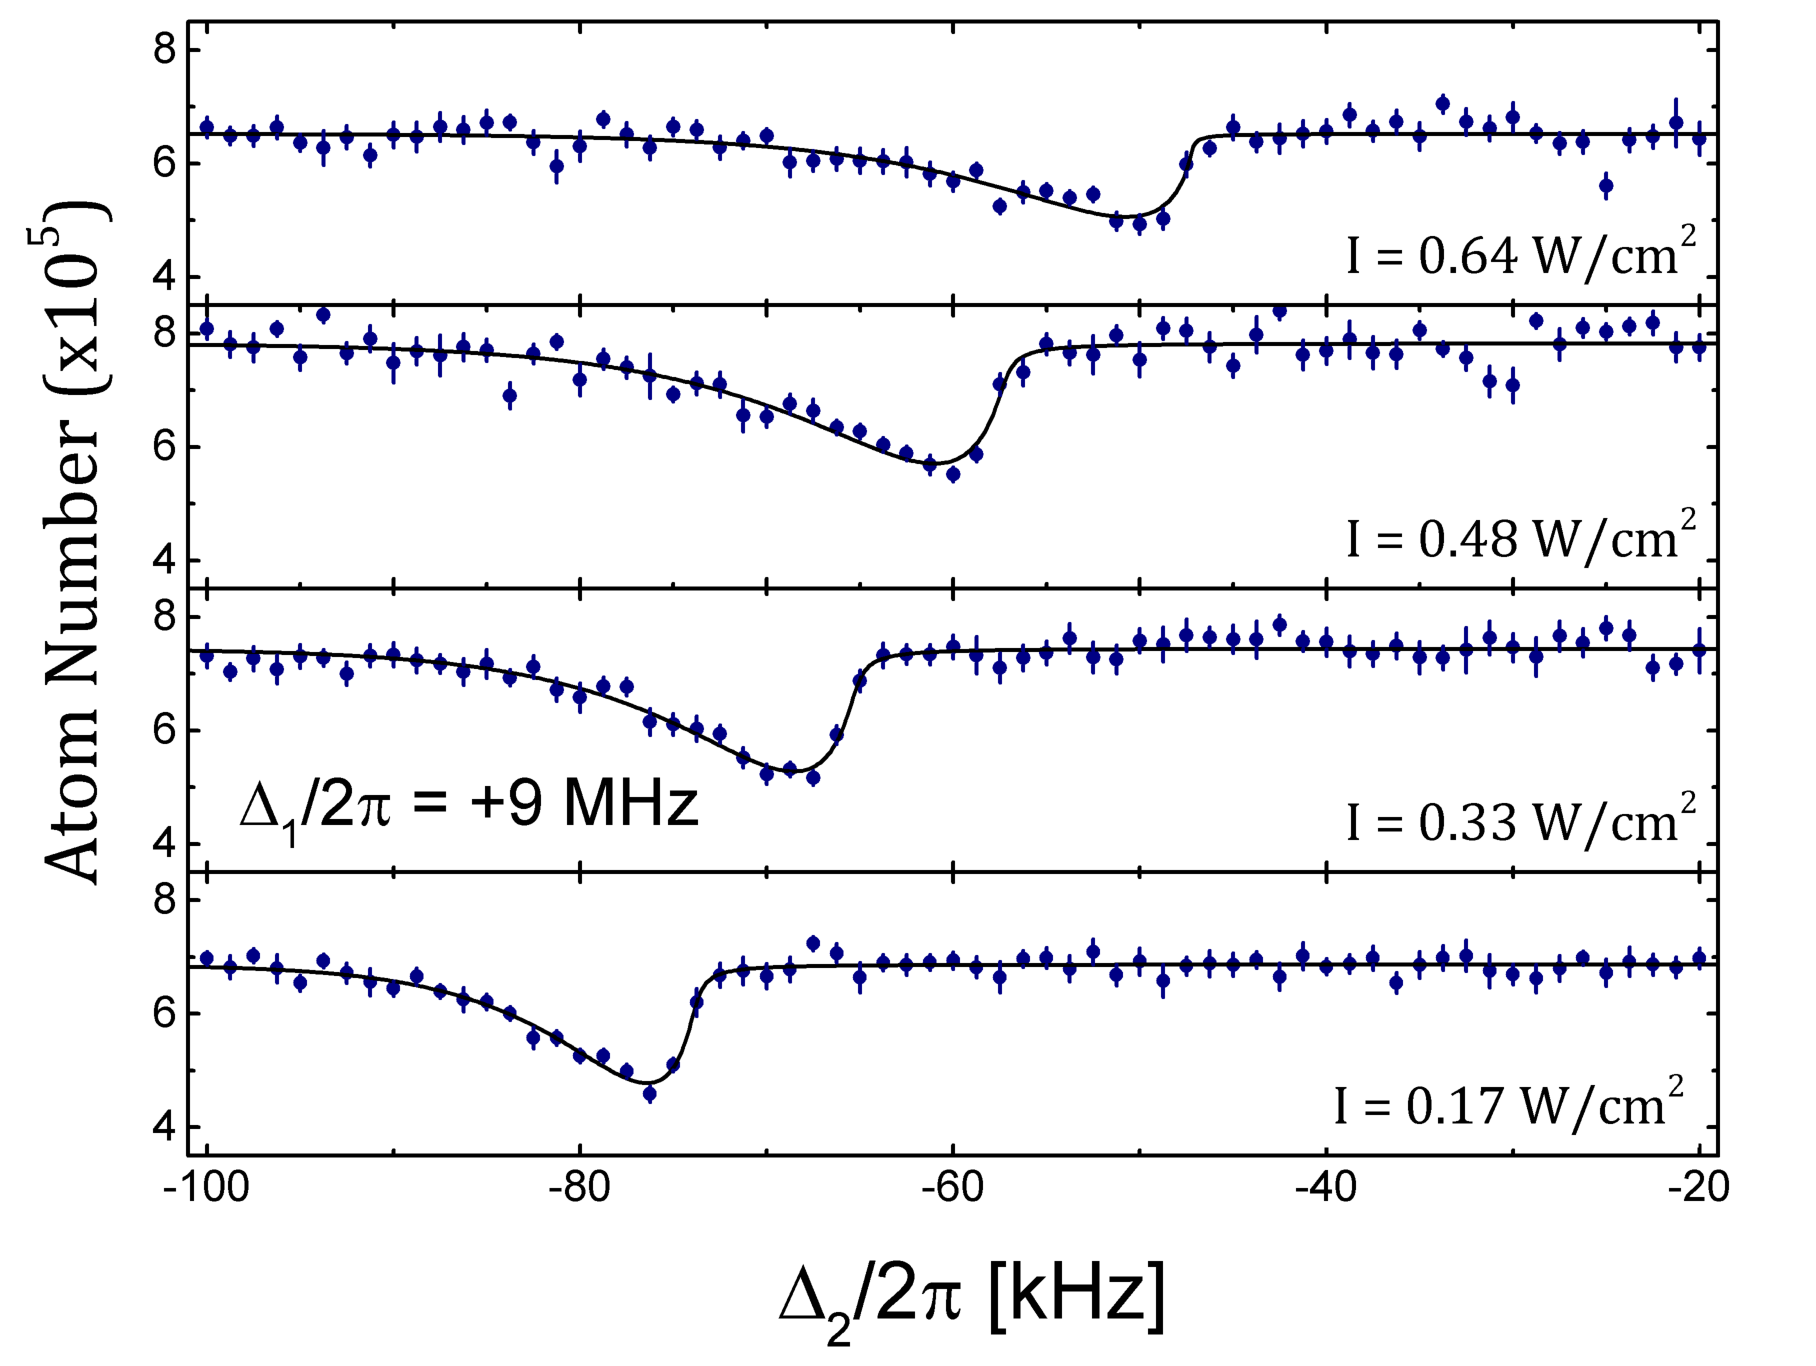
\includegraphics[width=\textwidth]{highIntSpectra.pdf}}
		\caption{Atom-loss spectra due to halo molecule spectroscopy}{The resulting atom number in the ODT following continuous exposure of the photoassociation lasers for exposure times on the order of several milliseconds at a fixed intermediate state detuning $\Delta_1/2\pi=+$9\,MHz. As the single-beam intensity $I$, is increased the atom-loss  lineshape noticeably shifts to lower binding energies. The procedure used to fit these lineshapes is discussed in the text.}
		\label{fig:highIntSpectra}
	\end{figure}
	
We model the rate of atom loss following the two-color PA theory of Bohn and Julienne and introduced in Sec.\,\ref{sec:bohn_and_julienne}.
Recall that the time-evolution of the total number of trapped atoms is given by Eq.\,\ref{eq:number}
\begin{equation*} \label{eq:4num}
   N(t)= \frac{N_0 \rm{e}^{-\Gamma t}}
   		{ 1 + \frac{2 N_0 \langle K \rangle V_2}{\Gamma V_1^2}(1-\rm{e}^{-\Gamma t}) }
\end{equation*}
with $\Gamma$ the one-body loss rate, $N_0$ the initial number of trapped atoms before applying the PAS lasers, and $V_q$ the effective volumes defined in Eq.\,\ref{eq:effectivevolumes}.
When fitting to experiments, we calculate the two-body average density distribution within the trap by considering the thermally averaged $\langle K \rangle_{\text{thermal}}$ (Eq.\,\ref{eq:twoPhotonKavg}) at each $\vec{r}$ contained within the trapping volume.
The trap averaged $\langle K \rangle_\text{trap}$ is given by
\begin{equation} \label{eq:chap4avgK}
	\langle K \rangle_\text{trap} = \frac{1}{V_2} \int_V e^{-2 U(\vec{r})/k_{B}T} \frac{1}{h\,Q_{T}} \int_{0}^{U_\text{depth}} d\epsilon \vert S \vert^2 \,e^{-\epsilon/k_{B}T}
\end{equation}
The partition function $Q_{T}=\left( \frac{2\pi k_{B}T \mu}{ h^2 }\right) ^{3/2}$ is determined for sample temperature $T$ and reduced mass $\mu = m/2$ with mass $m$ the mass of $\,^{86}$Sr.
We assume a fixed temperature throughout the exposure time.
Consideration of the temperatures measured from time-of-flight images showed no more than 15\% variation as $\Delta_2$ was scanned.
Finally, $U(\vec{r})$ is the trapping potential of the optical dipole trap and $U_{\text{depth}}$ is the overall trap depth defined in Sec.\,\ref{sssec:1064_modeling}.
For this analysis, a harmonic approximation was applied to $U(\vec{r})$.
This is an accurate representation of the trap when the ratio of trap depth to sample temperature is large, $U(\vec{r})/k_B T > 4$, as was true for these experiments.

We assume the dominant loss process to occur via the intermediate state $b_1$ and therefore use the scattering probability, $\vert S \vert^2 $ given in Eq.\,\ref{eq:twoPhotonSe1} 
\begin{equation} \label{eq:4sprob}
	\vert  S \vert^2 = \frac{(\Delta_2 + \epsilon/\hbar)^2 \gamma_1 \gamma_s}{
  	\left[ (\Delta_1+\epsilon/\hbar) (\Delta_2+\epsilon/\hbar)-\frac{\Omega_{12}^{2}}{4}\right]^2 + \left[ \frac{\gamma_1 + \gamma_s}{2}\right]^2 (\Delta_2+\epsilon/\hbar)^2}
\end{equation}
where ${\gamma}_{1}=2\gamma_{\text{atomic}}$, and $\gamma_{\text{atomic}}=4.7\times 10^4$\,s$^{-1}$ is the decay rate of the atomic $^3P_1$ level.
${\gamma}_{s}(\epsilon)$ is the stimulated width of $b_1$ due to coupling to the initial scattering state by the PAS lasers, which for low energy can be expressed as \cite{fks96,Bohn1996,Napolitano1994,bav00,Bohn1999}
\begin{equation} \label{equationstimulatedwidth}
	{\gamma}_{s}(\epsilon)=2k l_{\text{opt}} \gamma_1
\end{equation}
where the optical length ($l_{\text{opt}}\propto I_{689}$) is related to the overlap between the initial colliding state and $b_1$, and $k=\sqrt{2\mu \epsilon/ \hbar^2}$.
Our chosen intermediate state has optical length $l_{\text{opt}}/I=(1.5\pm0.3)\times 10^4\,a_0\mathrm{/(W/cm^2)}$ \cite{Borkowski2014a}, where $a_0=5.29\times 10^{-11}$\,m is the Bohr radius.

Since we are primarily concerned with measuring light shifts on the halo state, the statement of $\vert S \vert^2$ above omits any explicit inclusion of light shifts in contrast to the original theory.
This includes the shift of $b_1$ due to coupling to the ground state scattering continuum which was found to be a sufficient approximation for describing previous two-photon spectroscopy in $^{88}$Sr \cite{MartinezDeEscobar2008}.
Furthermore, lacking a model of coupling outside of our system, the scattering probability neglects dependence on shifts due to the trapping or photoassociation lasers coupling to states outside of this model.

The standard approach to describing photoassociation spectra is to consider the complete lineshape as a sum over Lorentzians shifted by the thermally distributed collision energy \cite{Julienne1989,Napolitano1994,Cote1995}.
However, Eq.\,\ref{eq:4sprob} is not a true Lorentzian due to the form of its dependence on $\Delta_2$.
We may recover the more intuitive approach to the lineshape by noting that for the experiments reported here, we maintain significant intermediate state detuning, $\Delta_1$, for which $|\Delta_1| \gg \Omega_{12}$.
Thus we are in the Raman regime and may further simplify Eq.\,\ref{eq:4sprob} by considering its behavior as a function of $\Delta_2$.
A maximum for this function occurs when $\Delta_2 + \epsilon/\hbar = \Omega_{12}^2/4 \Delta_1$.
In the regime of this maximum Eq.\,\ref{eq:4sprob} behaves similarly to a Lorentzian, thus by restricting the range of $\Delta_2$ to be near two-photon resonance and maintaining $|\Delta_1| \gg \Omega_{12}, \gamma_1, \gamma_s$, we can approximate $\vert  S \vert^2$ by \cite{Pachomov2017, Pachomow2017a}.
\begin{equation}
 \vert S\vert^2 \approx \frac{A(\epsilon)}{\left( \Delta_2+\epsilon/\hbar-\frac{\Omega_{12}^{2}} {4(\Delta_1+\epsilon/\hbar)}\right)^2+\left[ {\Gamma_L(\epsilon)}/{2}\right]^2}
\end{equation}
where 
\begingroup
\addtolength{\jot}{1em}
\begin{align}
  A(\epsilon) &= \frac{\Omega_{12}^{4}\gamma_1 \gamma_s(\epsilon)}{16(\Delta_1+\epsilon/\hbar)^4} \\
  \Gamma_L(\epsilon) &= \frac{\Omega_{12}^{2}[\gamma_1 +\gamma_s(\epsilon)]}{4(\Delta_1+\epsilon/\hbar)^2}
\end{align}
\endgroup

There remains several concerns regarding this formulation of the Bohn and Julienne theory for our experiment.
First, it assumes an isolated intermediate state, which is not strictly a valid approximation due to the proximity of the intermediate state $b_1$ to the $^1S_0\,+\,^3P_1$ asymptote and to the $\nu = -1$ state.
%Second, because of the small decay rate $\gamma_1$ of the intermediate molecular state associated with metastable $^3P_1$ atomic state, we also expect that loss from the ground molecular state should not be neglected.
Second, Eq.\,\ref{eq:4sprob} is derived assuming only a single near-resonant laser beam along each leg of the two-photon transition.
This condition is clearly violated for two-photon spectroscopy to a halo state where $\omega_1 - \omega_2 \approx -E_{b2} \ll |\Delta_1|$.
Thus, we expect pairs of colliding atoms will experience inelastic scattering processes in both fields simultaneously which will contribute to the overall observed transition strengths and light shifts.
During the photoassociation exposure, the total $689\,\text{nm}$ intensity, $I_{\text{689}}$, oscillates with near $100$\% contrast according to $I_{\text{689}}=I_1+I_2+2\sqrt{I_1I_2}\cos \left[(\omega_1-\omega_2)t \right]=2I\left\{1+\cos \left[(\omega_1-\omega_2)t \right]\right\}$.
When fitting the spectra, we assume an ansatz dependence of the bound-bound coupling, $\Omega_{12} \propto \langle I_{689} \rangle^{1/2}$ where $\langle I_{689} \rangle$ is the time averaged intensity which neglects the interference term between the lasers.

In the absence of a more rigorous theory treating these effects, we analyze loss spectra using the effective expression given by Eq.\,\ref{4equationApproxLorentzian}, where the observed molecular binding energy, $E'_{b2}$, includes any perturbations due to AC Stark shifts.
\begin{equation}\label{4equationApproxLorentzian}
  \vert S \vert^2 = \frac{\Gamma_L(\epsilon)+\gamma_{\text{eff}}}{\Gamma_L(\epsilon)} \frac{\eta  A(\epsilon)} {\left(\omega_1-\omega_2+\epsilon/\hbar-E'_{b2}/\hbar\right)^2+\left[
  	\frac{\Gamma_L(\epsilon)+\gamma_{\text{eff}}}{2}\right]^2}
\end{equation}
This formulation of the $\vert S \vert^2$ has been further modified with two additional parameters, $\eta$ and $\gamma_{\text{eff}}$, while maintaining the required unit normalization of the scattering probability \cite{Quemener2012,Krems2009a}.
The additional width, $\gamma_{\text{eff}}$, was added to allow for broadening which may have been neglected in this treatment of the inelastic scattering.
The amplitude scaling parameter $\eta$ accounts for additional phenomenological loss that is typically measured during photoassociation \cite{Zelevinsky2006,Borkowski2014a,Kim2016,Nicholson2015a,Yan2013c,Theis2004,Blatt}.

When performing fits of the atomic loss lineshapes using Eqs.\,\ref{eq:4num}, \ref{eq:chap4avgK}, and \ref{4equationApproxLorentzian}, we utilize independently determined simulations of the trapping potential $U(\vec{r})$.
The sample temperature, $T$, is measured from the time-of-flight and used to characterize the energy distribution of $\langle K \rangle_\text{thermal}$.
As a check of our lineshape model, we allowed the sample temperature to vary as a fit parameter and found reasonable agreement between the temperature estimated by the asymmetric tail of the lineshape and the time-of-flight temperature.
However, this process makes the fitting routine proceed much more slowly so we generally fix it to the value measured via time-of-flight.
The one-body loss rate $\Gamma$ was also measured and found to be $\approx\!5$\,s$^{-1}$.
All other values such $\gamma_s$, $\gamma_1$, $\Omega_{12}$, etc. are calculated for each spectrum using known physical values or locally measured estimates.
Thus, the remaining parameters $E'_{b2}$, $N_0$, $\eta$, and $\gamma_{\text{eff}}$ are independently fit and estimated for each spectrum.

Note that for each set of experimental conditions, $I_{689}$ and $\Delta_1$, several scans of the photoassociation process were accumulated. 
When determining the parameter estimates, $E'_{b2}$, $N_0$, etc., for a specific set of conditions, we independently fit and extract the coefficient values from each of the individual scans.
Then calculate the average and standard error for each parameter for a given set of conditions, $I_{689}$ and $\Delta_1$.

In this work, we are primarily concerned with variation of the halo resonance energy with the excitation laser intensity and intermediate state detuning as shown in Fig.\,\ref{fig:neuHalo}.
The estimate of $E'_{b2}$ from the spectra is largely determined by the sharp edge on the blue side of the spectrum.
While we cannot determined if the halo resonance energies are sensitive to other interactions causing shifts of the halo state, we do observe a striking dependence on the 689\,nm excitation intensity, $I_{689}$, as demonstrated in Figs.\,\ref{fig:highIntSpectra} \& \ref{fig:neuHalo}.
The relationship between the measured resonance positions and the unperturbed binding energy $E_{b2}$ is modeled as
\begin{equation}\label{Eq:4GlobalFit}
	E'_{b2} = E_{b2} + h\chi_{689}I_{689}
\end{equation}
We characterize the change in the AC Stark shift due to varying $\Delta_1$, by estimating the rate of change of the halo resonance energy with respect to $I_{689}$ using the linear fitting function Eq.\,\ref{Eq:4GlobalFit}.
When fitting, only intensities which exhibit linear scaling are included for each value of $\Delta_1$.
This estimates the susceptibility of the halo state, $\chi_{689}(\Delta_1)$, which are plotted as a function of $\Delta_1$ in Fig.\,\ref{fig:neuHalo}.
	\begin{figure}
	\centerline{
	  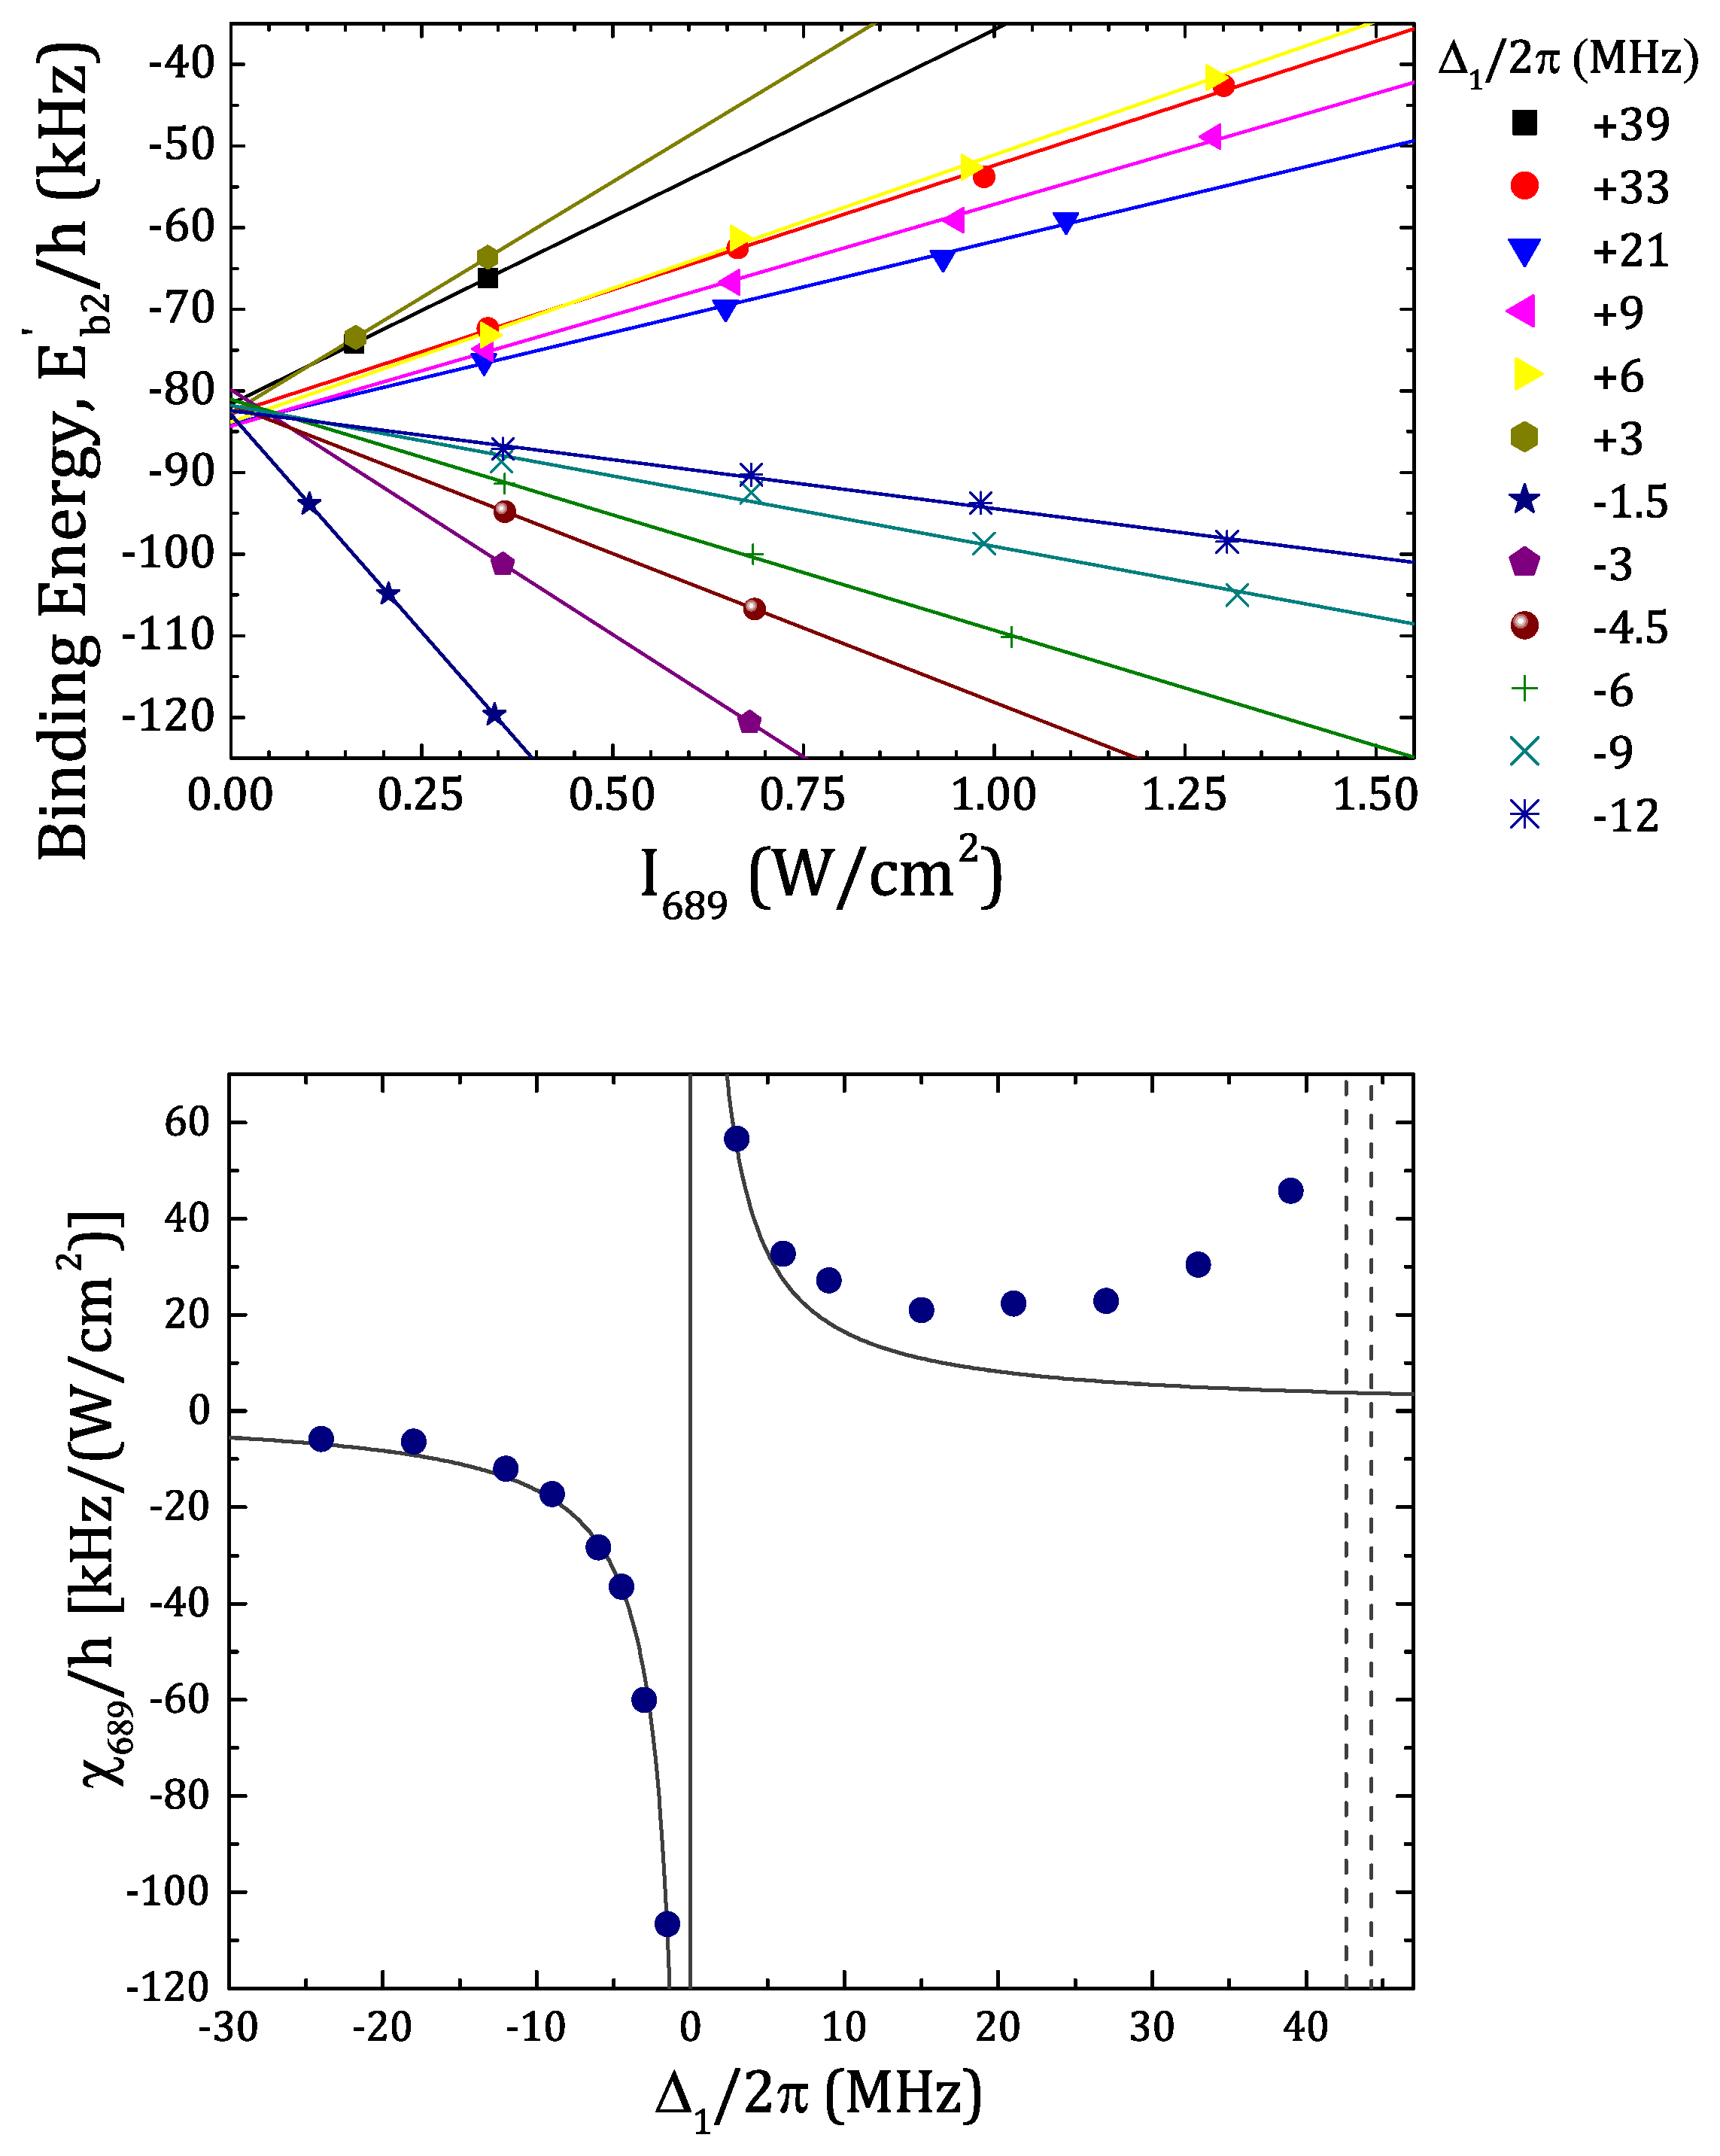
\includegraphics[width=0.75\textwidth]{neuHalo.pdf}}
	  \caption{Halo state resonances and susceptibilities, $\chi_{689}$}{Summary of the halo PAS experimental results. Top: A selection of two-photon PA resonance positions as a function of twice the single-beam excitation intensity, $I_{689} = 2I$, for various intermediate state detunings $\Delta_1$. The solid lines are fits used to determine $\chi_{689}$ at each detuning. Bottom: The susceptibility, $\chi_{689}$, across all intermediate state detunings probed in this study. Dashed lines indicate the positions of the $\nu=-1$, $J=1$ excited molecular state, bound by $1.633(1)$\,MHz, and the $^1S_0\,+\,^3P_1$ continuum. Dark solid line is a guide to the eye $\propto 1/\Delta_1$.}
	   \label{fig:neuHalo}
	\end{figure}
	
%Specifically, we estimated the value of the bound-bound Rabi frequency, $\Omega_{12}/2 \pi \sim 850$\,kHz after performing a preliminary analysis of the frequency dependence of the binding energy over all of the data.
%Subsequently, this R	
%	
%While useful for a general description, the effective form of Eq.\,\ref{equationApproxLorentzian} fails to identify contributing factors to the overall observed loss and thus little may be rigorously concluded about the coefficient estimates of $\eta$ and $\\gamma_{\text{eff}}$.
	
%We also neglect shifts due to collisions and the trapping laser, which are small at the large excitation-laser intensities used here.	
%	
%Eq.\,\ref{equationSprob} neglects lights shifts due to the trapping lasers or caused by the PA lasers coupling to states outside of our model.
%
%Light shifts due to the trapping lasers and collisions with ground-state atoms (density $n$) should contribute to shifts of molecular resonance.	
%	
%%Subsequent modeling validated this assumption, which we discuss shortly.
%
%which will contribute to the observed transition strength and light shifts of the levels.
%
%First, when fitting the lineshape, $\Delta_1$ is fixed for all values of $\Delta_2$ which neglects any variation of the AC Stark shift with $\omega_2$.
%
%We expect that both 689\,nm excitation lasers will contribute to shift the halo state resonance.
%
%
%
%, which is not a good approximation for two-photon spectroscopy of a halo state and the resulting small laser frequency difference 
%
%Although Eq.\,\ref{eq:4sprob} may appear a Lorentzian, the inclusion of $\Delta_2$ in both terms of the denominator can result in a long tail 
%
%Further insight into the behavior of the scattering probability in Eq.\,\ref{equationSprob} 
%
%displays a maximum near two-photon resonance at $\Delta_2+\epsilon/\hbar =\Omega_{12}^2/4\Delta_1$.
%
%if the detuning is restricted to near two-photon resonance then $\vert S\vert^2$ can be approximated as a Lorentzian
%
%derived for two well separated lasers
%approximate decay from b2 with an additional width factor
%temps agreed
%	
	
	
\section{Frequency dependence of the binding energy} \label{sec:highE_theory}		
Collaborating with Kon Wen Yu, of the Hazzard group, the data shown in Fig.\,\ref{fig:neuHalo} was used to develop and assess several theoretical descriptions in order to reproduce and predict the resonance positions and susceptibility of the halo molecule state.
Additionally, we evaluated the effect of the two-frequency drive on the observed halo resonance energies and reproduced the emergence of higher-order loss processes observed in the experiment.

These theoretical approaches began with the setup and numerical evaluation of a time-dependent three-level system.
This model was then analyzed using Floquet and perturbation theory to develop an approximate analytic formula for predicting the halo resonance shift.
Throughout this analysis, we neglect the motional degrees of freedom for the initial state of two free atoms.
This greatly simplifies the physical processes we must consider and allows us to deduce an analytic result for the scaling of the binding energy.
%A more complete description of the multi-channel scattering problem may be developed using a fully coupled-channel calculation.
%However, development of such a model is beyond the scope of the present work.
For the remainder of this chapter, our discussion will focus on the results of Yu's analyses and leave the details of his derivation to Ref.\,\cite{Kon2018}.

The photoassociation experiment is modeled using a three-level system composed of two well-separated atoms \ket{0}, an intermediate dimer state in an excited electronic potential \ket{b1}, and a dimer in the ground electronic state \ket{b2}.
This setup is outlined in Fig.\,\ref{fig:PASDiagram} where we have defined \ket{0} to be a pair of atoms with $\epsilon=0$ relative collision energy.
The Hamiltonian for this system is

\begin{equation} \label{eq:3LvlModel}
\hspace*{-1cm} 
	H=
    \begin{bmatrix}
      0 & \Omega_{1,01}\mathrm{cos}(\omega_1 t) + \Omega_{2,01}\mathrm{cos}(\omega_2 t) & 0 \\
      \Omega_{1,01}\mathrm{cos}(\omega_1 t)+ \Omega_{2,01}\mathrm{cos}(\omega_2 t) & E_{b1} - \imath \frac{\Gamma_1}{2} & \Omega_{1,12}\mathrm{cos}(\omega_1 t)+ \Omega_{2,12}\mathrm{cos}(\omega_2 t) \\
      0 & \Omega_{1,12}\mathrm{cos}(\omega_1 t)+ \Omega_{2,12}\mathrm{cos}(\omega_2 t) & E_{b2} - \imath \frac{\Gamma_2}{2} \\
    \end{bmatrix}
\end{equation}

\bigskip
Unlike the typical $\Lambda$-model considered in the Bohn and Julienne formalism, Eq.\,\ref{eq:3LvlModel} considers both lasers 1 and 2 to drive the transition $\ket{0}\,\rightarrow\,\ket{b1}$ and $\ket{b1}\,\rightarrow\,\ket{b2}$.
%We denote the coupling of a specific laser acting on a particular transition with the notation $\Omega_{\text{laser, initial}\,\rightarrow\,\text{final}}$.
Decay terms are included to describe atom loss with $\Gamma_1$ representing spontaneous emission from the intermediate bound state due to natural decay and $\Gamma_2$ representing loss from the halo state due to collisions with background atoms.

The time-evolution of Eq.\,\ref{eq:3LvlModel} begins in \ket{0} and proceeds for a time $\tau$ using similar optical couplings and oscillating optical intensity as present during the photoassociation experiments.
The model is numerically solved to generate a simulated spectrum as shown in Fig.\,\ref{fig:haloResProcess}.
From these spectra, we estimate the halo resonance energy by determining the frequency of peak loss.
The results of these simulations are shown in Fig.\,\ref{fig:3LvlModel}.
	\begin{figure}
		\centerline{
		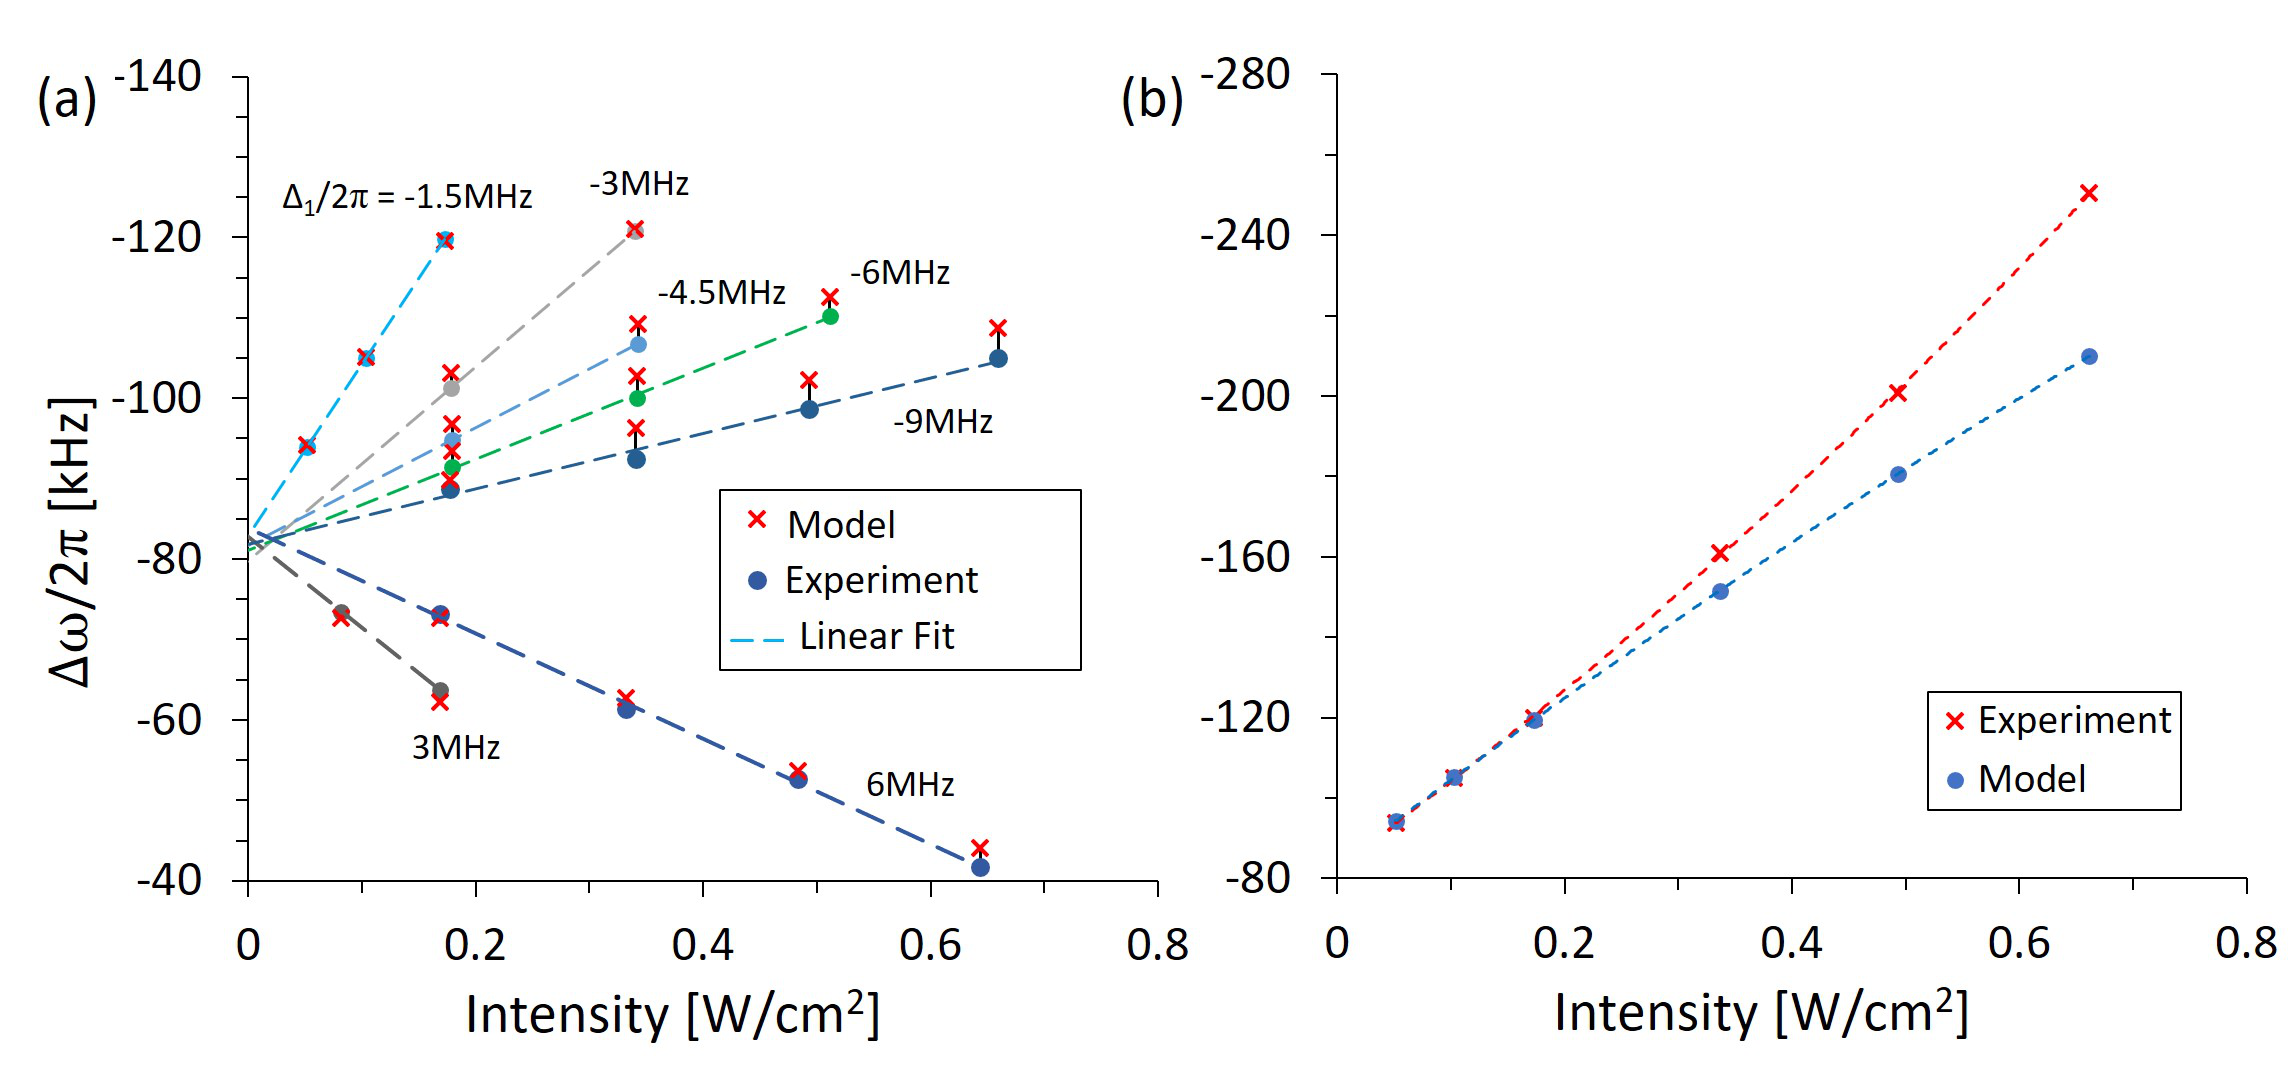
\includegraphics[width=\textwidth]{threeLevelModel.png}}
		\caption{Comparison of a three-level model to experimental halo PAS}{a) The resonance energies, E$_{b2}'$, determined from  the experiments as well as the corresponding predicted resonance position from numerical simulation of three-level model given by Eq.\,\ref{eq:3LvlModel}. This is the same data and linear fits as shown in Fig.\,\ref{fig:neuHalo}. b) Binding energy positions for $\Delta_1/2 \pi = -$1.5\,MHz data over a larger range of intensities for which the experimental results are not well described by linear scaling as predicted by the three-level model. Quadratic fits are shown as a guide to the eye.}
		\label{fig:3LvlModel}
	\end{figure} 
The predicted halo resonance energies generally agrees with experimental data and reproduces a linear scaling of the binding energy consistent with the experimental observations.
This indicates that effects missing from this theory – the motion of the atoms \cite{Bohn1996,Bohn1999}, interaction shifts due to molecules and atoms scattering off of other molecules and atoms \cite{wfh00}, and the varying density within the trap \cite{MartinezDeEscobar2008} – are not necessarily relevant for considering the effects of the two-frequency drive and determination of the internal interaction strengths.
%For some combinations of intensity and $\Delta_1$ there is reasonable agreement between the model and the data.

However, as intensity is increased the model begins to deviate from the experimental data, limiting its regime of applicability.
Fig.\,\ref{fig:highIntSpectra}b shows an example where the three-level model tends to underestimate the resonance energy at higher intensities.
This behavior is suggestive of additional interactions between the halo molecule state and one or more levels outside of our model.

We expect the predictive capability of the three-level system to prove useful for future studies of the $^{86}$Sr halo molecule.
Although, the numerical time-evolution is intensive and would require solving multiple simulations when including the halo resonance energy in the development of future theories.
Thus, to obtain analytic insight into the three-level model, the Hamiltonian of Eq.\,\ref{eq:3LvlModel} was treated under Floquet theory.
We leave the details of this analysis to Ref.\,\cite{Kon2018} but note that once the Floquet Hamiltonian has been found, a perturbative expansion can be applied in the region around $|\omega_1 - \omega_2| \approx -E_b^0$ by assuming $|\Delta_1| \gg \Omega_{01}, \Omega_{12}, \Delta_2, |\omega_1 - \omega_2|$, where $\Delta_2 = \omega_1 - \omega_2 - E_b^0$.
Additionally, we assume $\Omega_{12} \gg \Omega_{01}$.
The resulting expression for the shift of the halo resonance energy is then
\begin{equation} \label{eq:floquetShift}
	\Delta \omega = \frac{\Omega^2}{4} \left( \frac{1}{\Delta_1 + E_b^0 + \Delta\omega} + \frac{1}{\Delta_1 + E_b^0} \right)
\end{equation}
where $\Delta\omega$ is the shift from the natural binding energy $E_b^0$ and we have defined $\Omega_{1,12}=\Omega_{2,12}=\Omega$ in the case that $I_1=I_2$.
Comparison of this analytic formula with results from the numerical simulations show excellent agreement, even outside the region of strict validity of the perturbative expansion.
Eq.\,\ref{eq:floquetShift} also confirms our initial hypothesis, applied when fitting the halo molecule lineshapes in the previous section, that the AC Stark shift scales as nearly twice the single-beam intensity.
This is consistent with approximations of light shifts made in previous similar experiments \cite{Wynar2000,Tojo2006}.

As an application of Eq.\,\ref{eq:floquetShift}, we note that $\frac{d \Delta\omega}{d I}$ gives the susceptibility $\chi_{689}(\Delta_1)$ of the halo state.
Fig.\,\ref{fig:floquetFitChi} plots the analytic susceptibility over $\Delta_1$ resulting from fitting the coupling parameter in $\frac{d \Delta\omega}{d I}$.
	\begin{figure} 
	\centerline{
	  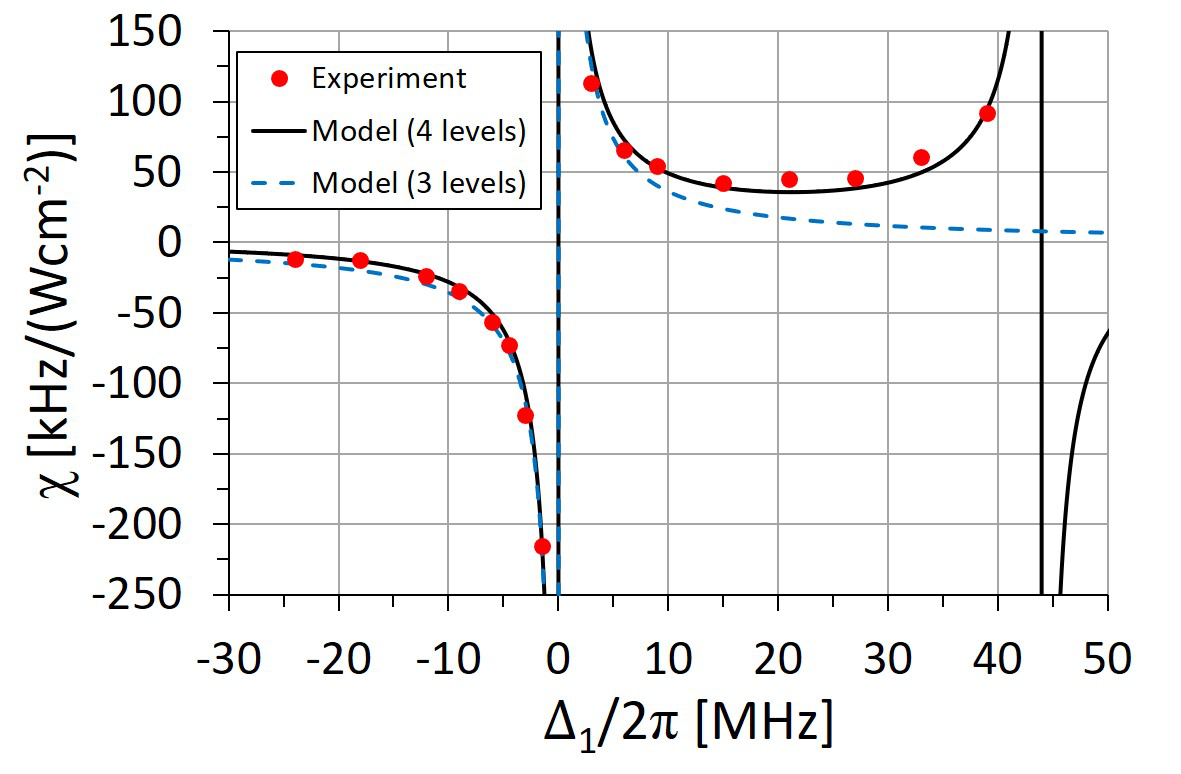
\includegraphics[width=\textwidth]{variationOfDelta1.png}}
	  \caption{Analytic approximation of the susceptibility}{Plot of the experimental susceptibility data shown in Fig.\,\ref{fig:neuHalo}. These points are fit with the analytic susceptibility predicted from the Floquet treatment of the three-level and four-level models. The coupling from the four-level model is estimated to be $\Omega_{12}/2\pi=850$\,kHz for $I=1$\,W/cm$^2$}
	  \label{fig:floquetFitChi}
	\end{figure}
Once more we see that the three-level model cannot reproduce the experimental observations as intermediate state detuning is increased.
This is most likely due to coupling with the $\nu=-1$, $J=1$ excited molecular state and the $^1S_0\,+\,^3P_1$ continuum.
Experimentally we were unable to isolate and determine the separate effects of these states.
Thus, as an approximate theoretical approach, the three-level model is extended with a virtual fourth-level, \ket{X}, specified by
\begin{equation} \label{eq:addXLvl}
	H'=H_0 + E_X\ket{X}\bra{X} + \left[ \Omega_{1,0X}\cos(\omega_1t) + \Omega_{2,0X}\cos(\omega_2t) \right] \ket{0}\bra{X} + \text{h.c.}
\end{equation}
where $H_0$ is the three-level Hamiltonian in Eq.\,\ref{eq:3LvlModel}.
The virtual state \ket{X} may, in general, having couplings $\Omega_{0X}$ and $\Omega_{2X}$.
We choose to set $\Omega_{2X} = 0$ in Eq.\,\ref{eq:addXLvl} and consider the dominant coupling as being between states \ket{0} and \ket{X}.
This approximation is motivated by the positive slope of the observed susceptibilities as $\Delta_1$ is varied towards the $^1S_0\,+\,^3P_1$ asymptote which suggests that the ground state is shifting faster than the halo state.
If instead we assumed that $\Omega_{2X} \gg \Omega_{0X}$, the sign of the AC Stark shift would be negative at red-detuning, which is inconsistent with our observations.
Additionally, we choose to set the energy of the virtual state to the energy of the $^1S_0\,+\,^3P_1$ asymptote, $E_X = E_{b1} + 2\pi\hbar \times 44.2$\,MHz.

A fit of the Floquet treatment of the four-level model is shown in Fig.\,\ref{fig:floquetFitChi} and yields $\Omega_{12}/2\pi=850$\,kHz for $I=1$\,W/cm$^2$.
Note that $\Omega_{12}$ as defined here would be the splitting of the Autler-Townes doublet \cite{MartinezDeEscobar2008, Pachomow2017a}, which differs from the Bohn-Julienne definition of the molecular Rabi coupling \cite{Bohn1996,Bohn1999}.

Using the measured $\Omega_{12}$, one can extract the Franck-Condon factor, $f_{\text{FCF}}$, reflecting the overlap of the ground and intermediate molecular states through
\begin{equation}\label{Eq:FranckCondonRabiFrequency}
	\Omega_{12}=\sqrt{f_{\text{ROT}}}\sqrt{f_{\text{FCF}}}\gamma_{\text{atomic}}\sqrt{\frac{I}{2 I_{\text{sat,atom}}}}
\end{equation}
where $I_{\text{sat,atom}}=2\pi^2\hbar c \gamma_{\text{atomic}}/(3\Lambda^3)=3$\,$\mu$W/cm$^2$ is the atomic saturation intensity for the $^1S_0\,\rightarrow\,^3P_1$ transition and $I=I_{689}/2$ is the single-beam intensity.
The rotational factor $f_{\text{ROT}}$ accounts for the change in dipole moment from atom to molecule due to symmetry of the wave function and projection on a rotating molecular axis.
Following the formalism described in \cite{Reschovsky2018,Pachomow2017a}, $f_{\text{ROT}}=2$ for the $J=1\rightarrow 0$ bound-bound molecular transition studied here.
This yields $f_{\text{FCF}} = 0.03$.

%At the range of intensities and detunings shown in Fig. 2(a), we observe that the three-level model generally yields a linear relation between binding energy and intensity.
%However, deviations between experiment and model binding energies are observed at higher intensity values for small detuning (when ac Stark shift is large), as shown in Fig. 2(b).
%
%Considering only low-intensity data where the binding energy varies linearly with intensity, Fig. 3 shows that there are deviations between susceptibility predicted by 8 the three-level model and experimental results when the detuning is large.
%This may be due to the presence of another level X. 
%
%Although this should not be construed as strong evidence for an additional level at this energy, it does suggest that additional levels at high energies are a candidate cause for this effect.
%Understanding the frequency-dependence of $\chi_{689}$ is important for investigating this possibility, so we extracted this parameter from spectra at a wide range of 689-nm laser intensities and detuning from the intermediate resonance ($\Delta_1$).

%consider the scaling of the halo binding energy with intensity in a region where the three-level model is accurate.
%For $\Omega_{i,01}\ll \Omega_{i,12} \ll |\Delta_{1}|\equiv |\omega_1-E_{b1}/\hbar|$, which is analogous to the experimental conditions in the isolated resonance regime, we find that the two-photon resonance is shifted by
%\begin{equation}\label{Eq:ACStarkFullModel}
%	\frac{\hbar\Omega_{1,12}^{2}}{4\Delta_{1}}+\frac{\hbar\Omega_{2,12}^{2}}{4\left(\Delta_{1}-E_{b2}/h\right)}\approx
%	\frac{\hbar\Omega_{12}^{2}}{2\Delta_{1}}.
%\end{equation}
%where we have assumed that $\Omega_{1,12} \approx \Omega_{2,12}$.

%
%Thus, the susceptibility is related to the Rabi frequency for a single-beam intensity $I$ through $\chi_{689}\approx(\Omega_{12}/\sqrt{I})^2/(8\pi \Delta_1)$.

\section{Multi-photon loss processes} \label{sec:highE_coupling}
	\begin{figure} 
	\centerline{
	  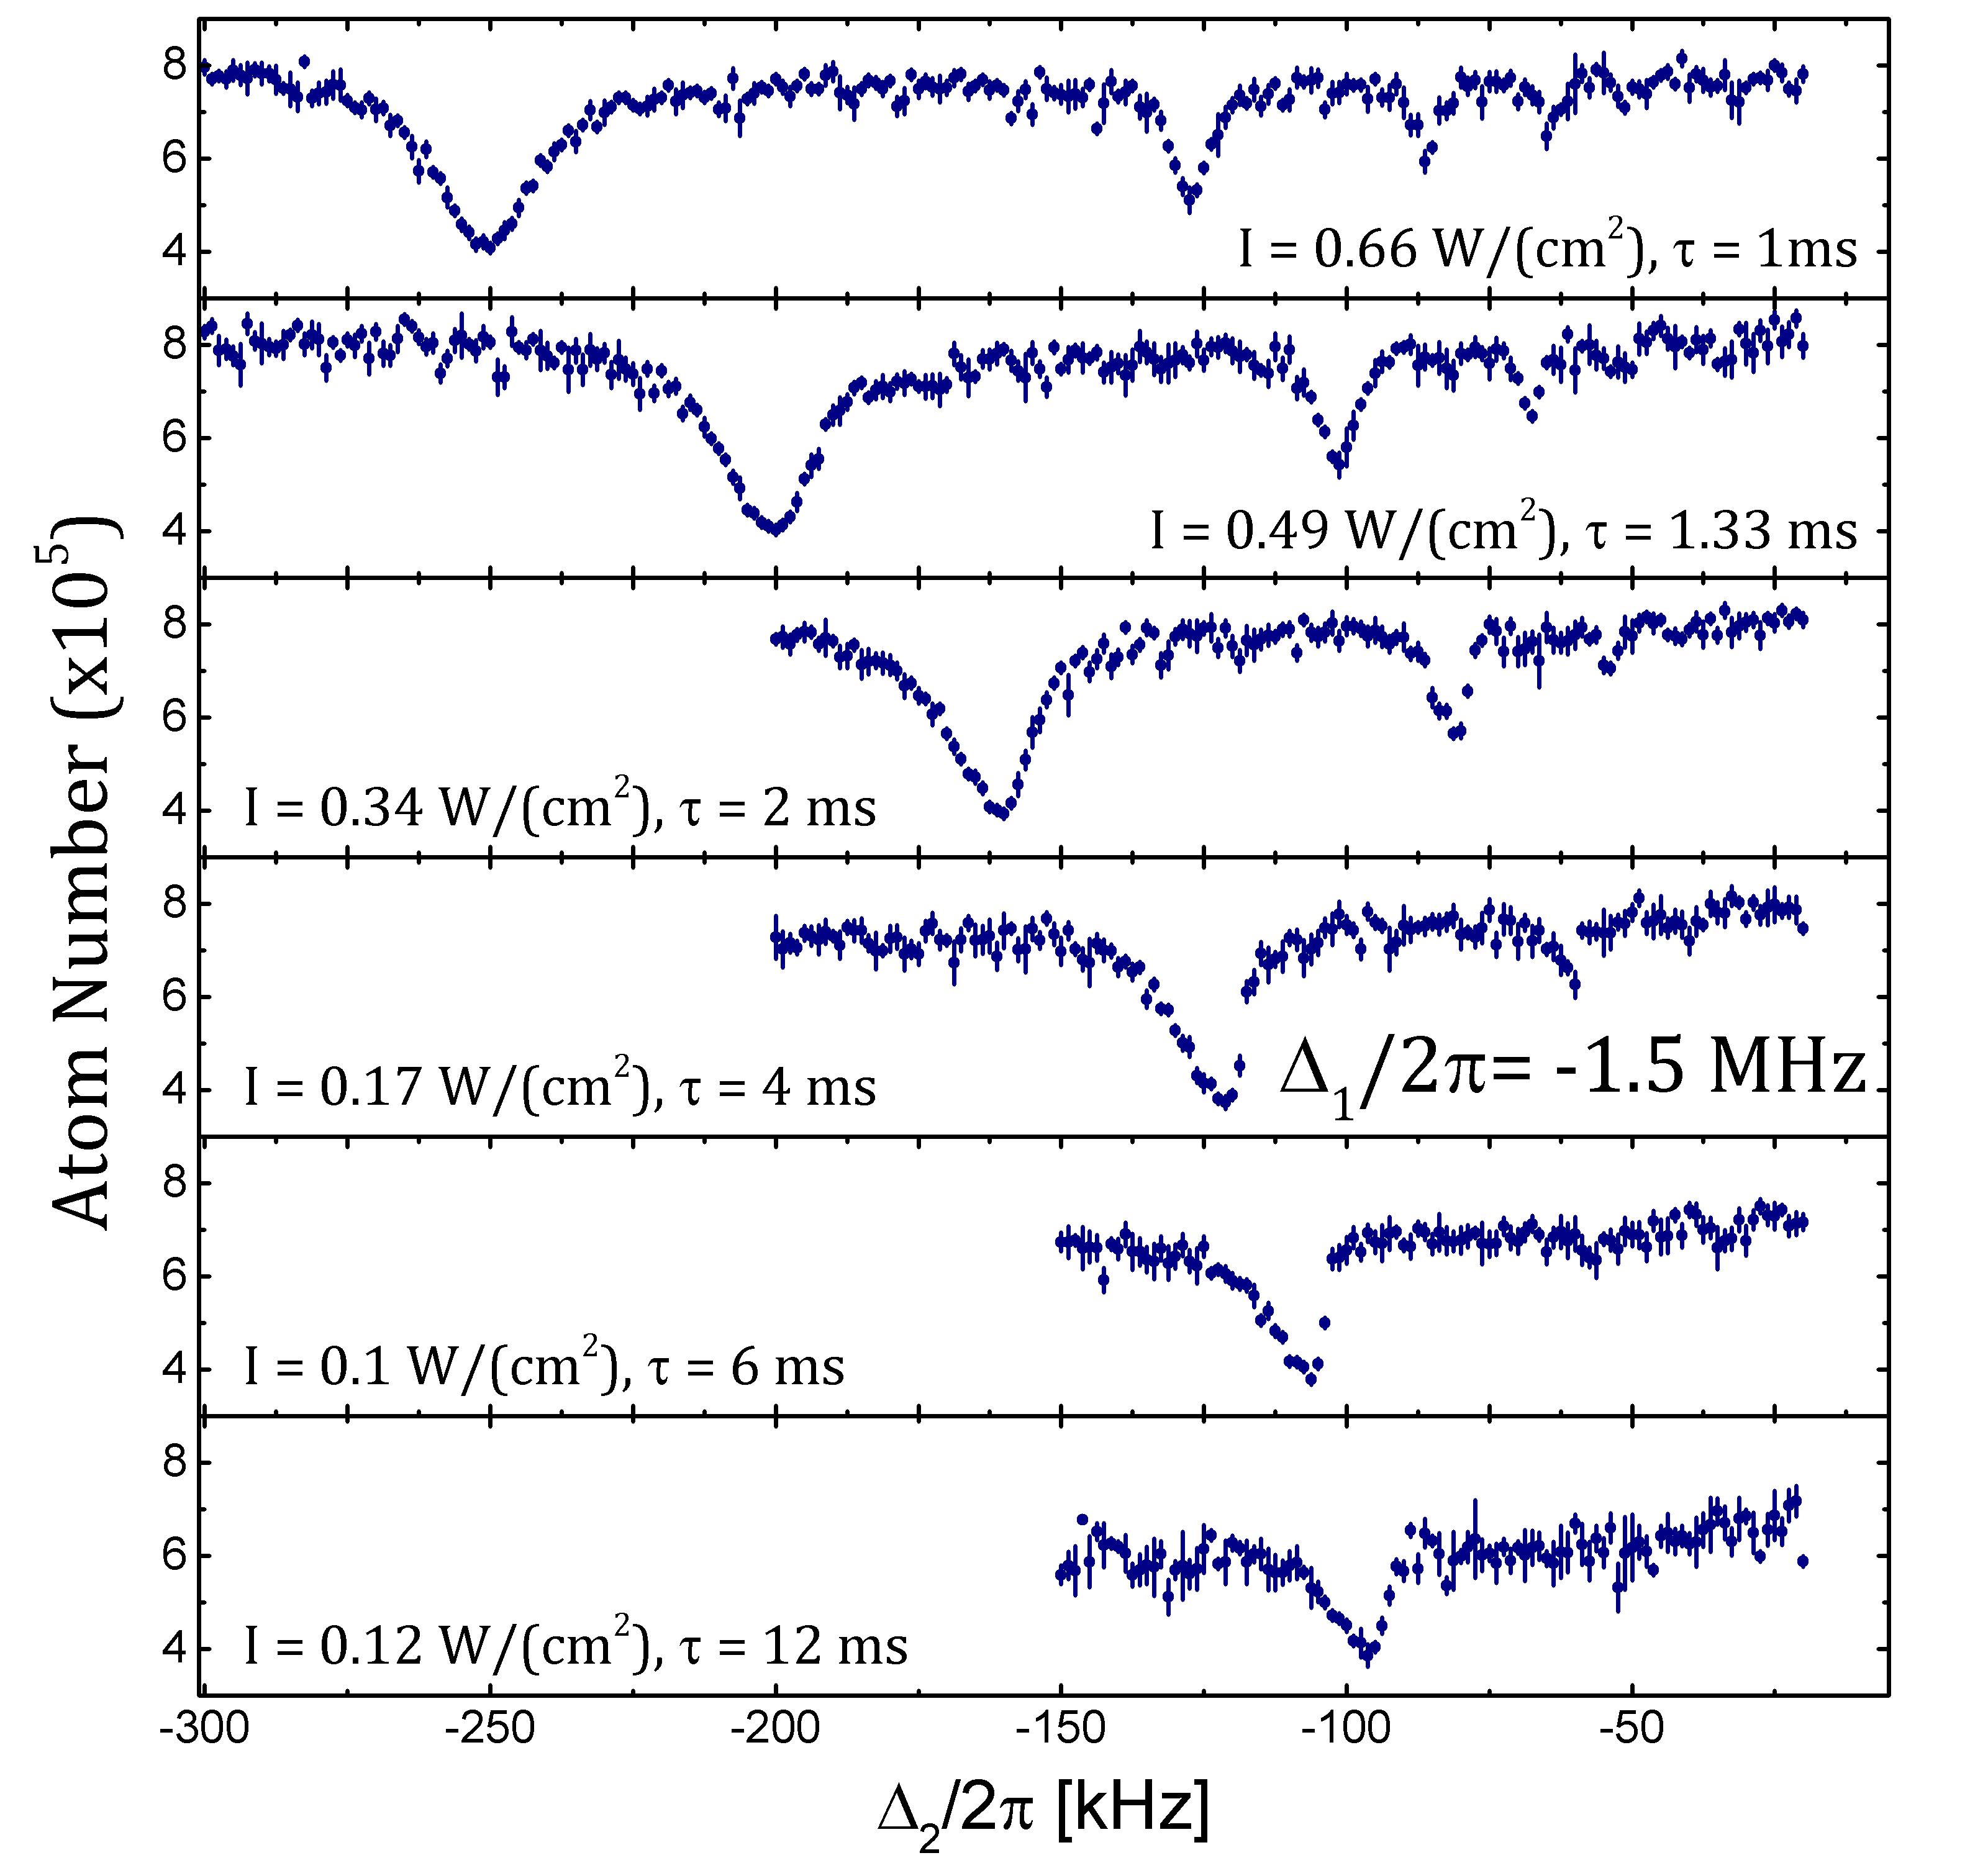
\includegraphics[width=1.1\textwidth]{Higher_Order Raman_vsInt.png}}
	  \caption{Observation of higher order Raman processes}{}
	  \label{fig:highIntMultiPhoton}
	\end{figure}
In the regime of strongest coupling between the halo state and intermediate excited molecular state, we observe the emergence of higher order loss features absent in the typical $\Lambda$-model due to the separability of the excitation lasers. %where the lasers are well separated in frequency and therefore drive each transition independently.
Fig.\,\ref{fig:highIntMultiPhoton} shows a series of spectra close to resonance which demonstrates the appearance of these loss features.
At low-intensity a single prominent PAS lineshape around $\Delta_2 \approx -100$\,kHz is observed.
Then, as the intensity is increased, the resonance energy of the primary loss feature, defined as $E_{b2}$, shifts significantly more deeply into the ground state potential.
%due the the large bound-bound coupling strength, $\Omega_{12}$.
Accompanying this shift, additional loss features continue to emerge in the spectrum as the intensity is further increased. These satellite features also appear to scale with intensity and the position of the primary loss feature.
Increasing intensity also results in an increase in the linewidth as the lineshape broadens from an asymmetric feature into a fully symmetric profile.
This is indicative of power broadening of the two-photon transition as population is cycled between the halo and continuum states.

Two conclusions may be drawn from these spectra that are of particular note.
First, the shift of the halo state to a binding energy of $\approx$250\,kHz for the highest intensity spectrum represents a significant change in the scattering length of freely scattering atoms in the $^1S_0\,+\,^1S_0$ continuum.
In the next chapter, we will discuss our precise determination of the halo molecule resonance energy which we measure to be E$_{b2}=-83$\,kHz.
Presuming this value of E$_{b2}$ for the moment, we can estimate the change in scattering length due to a $250$\,kHz change in the halo state resonance energy using E$_{b2}=-\hbar^2/(2 \mu a^2)$, where $\mu$ is the reduced mass of the strontium-86 halo molecule and $a$ is the $s$-wave scattering length.
From the highest intensity spectrum, the primary loss feature is shifted by approximately $3\times$ the natural binding energy.
This reduces the $86$-$86$ scattering length to $\sim$500\,a$_0$, or approximately $60$\% of its natural value.
The proximity of $^{86}$Sr to a scattering resonance and the susceptibility of the halo binding energy to the intensity of the excitation light suggests using light to tune the binding energy and scattering length as was done with optically assisted magnetic Feshbach resonances \cite{blv09,chx15}
This compliments previous work on the use of optical Feshbach resonances in strontium \cite{fks96,Theis2004,Yamazaki2010,Blatt,Yan2013c}. 

Second, consideration of the peak loss positions in Fig.\,\ref{fig:highIntMultiPhoton} shows that each higher order process is related to the position of the primary loss by approximately $E_{b2}/2$. $E_{b2}/3$, $\dots$.
This scaling suggests a non-linear process whereby multiple photons from the excitation light fields are absorbed and emitted to reach the final state.
This is possible because of the small overall detuning, $\Delta_2$, and strong coupling between the halo and intermediate state.
This hypothesis can be tested using time-evolution of the three-level model to predict the spectra under similar conditions.
Fig.\,\ref{fig:multiPhotonTheory} shows a schematic example of the multi-photon process as well as the result of the numerical evaluation for a selection of the strongly coupled spectra shown in the previous figure.
Despite its simplicity, the three-level model captures the relevant physics and accurately predicts the emergence of multi-photon loss features near the positions of the experimentally measured loss.
%Such higher order process are therefore inherent in similar systems and are not due to the excitation to the halo molecule.
Furthermore, at high-intensity, this model reproduces the symmetric lineshape profile indicating that power broadening is becoming the dominant source of the width.
This shows that at high-intensity, the scattering nature of the problem, in which the initial state is embedded in a continuum of free atoms, is relatively unimportant.
	\begin{figure} 
	\centerline{
	  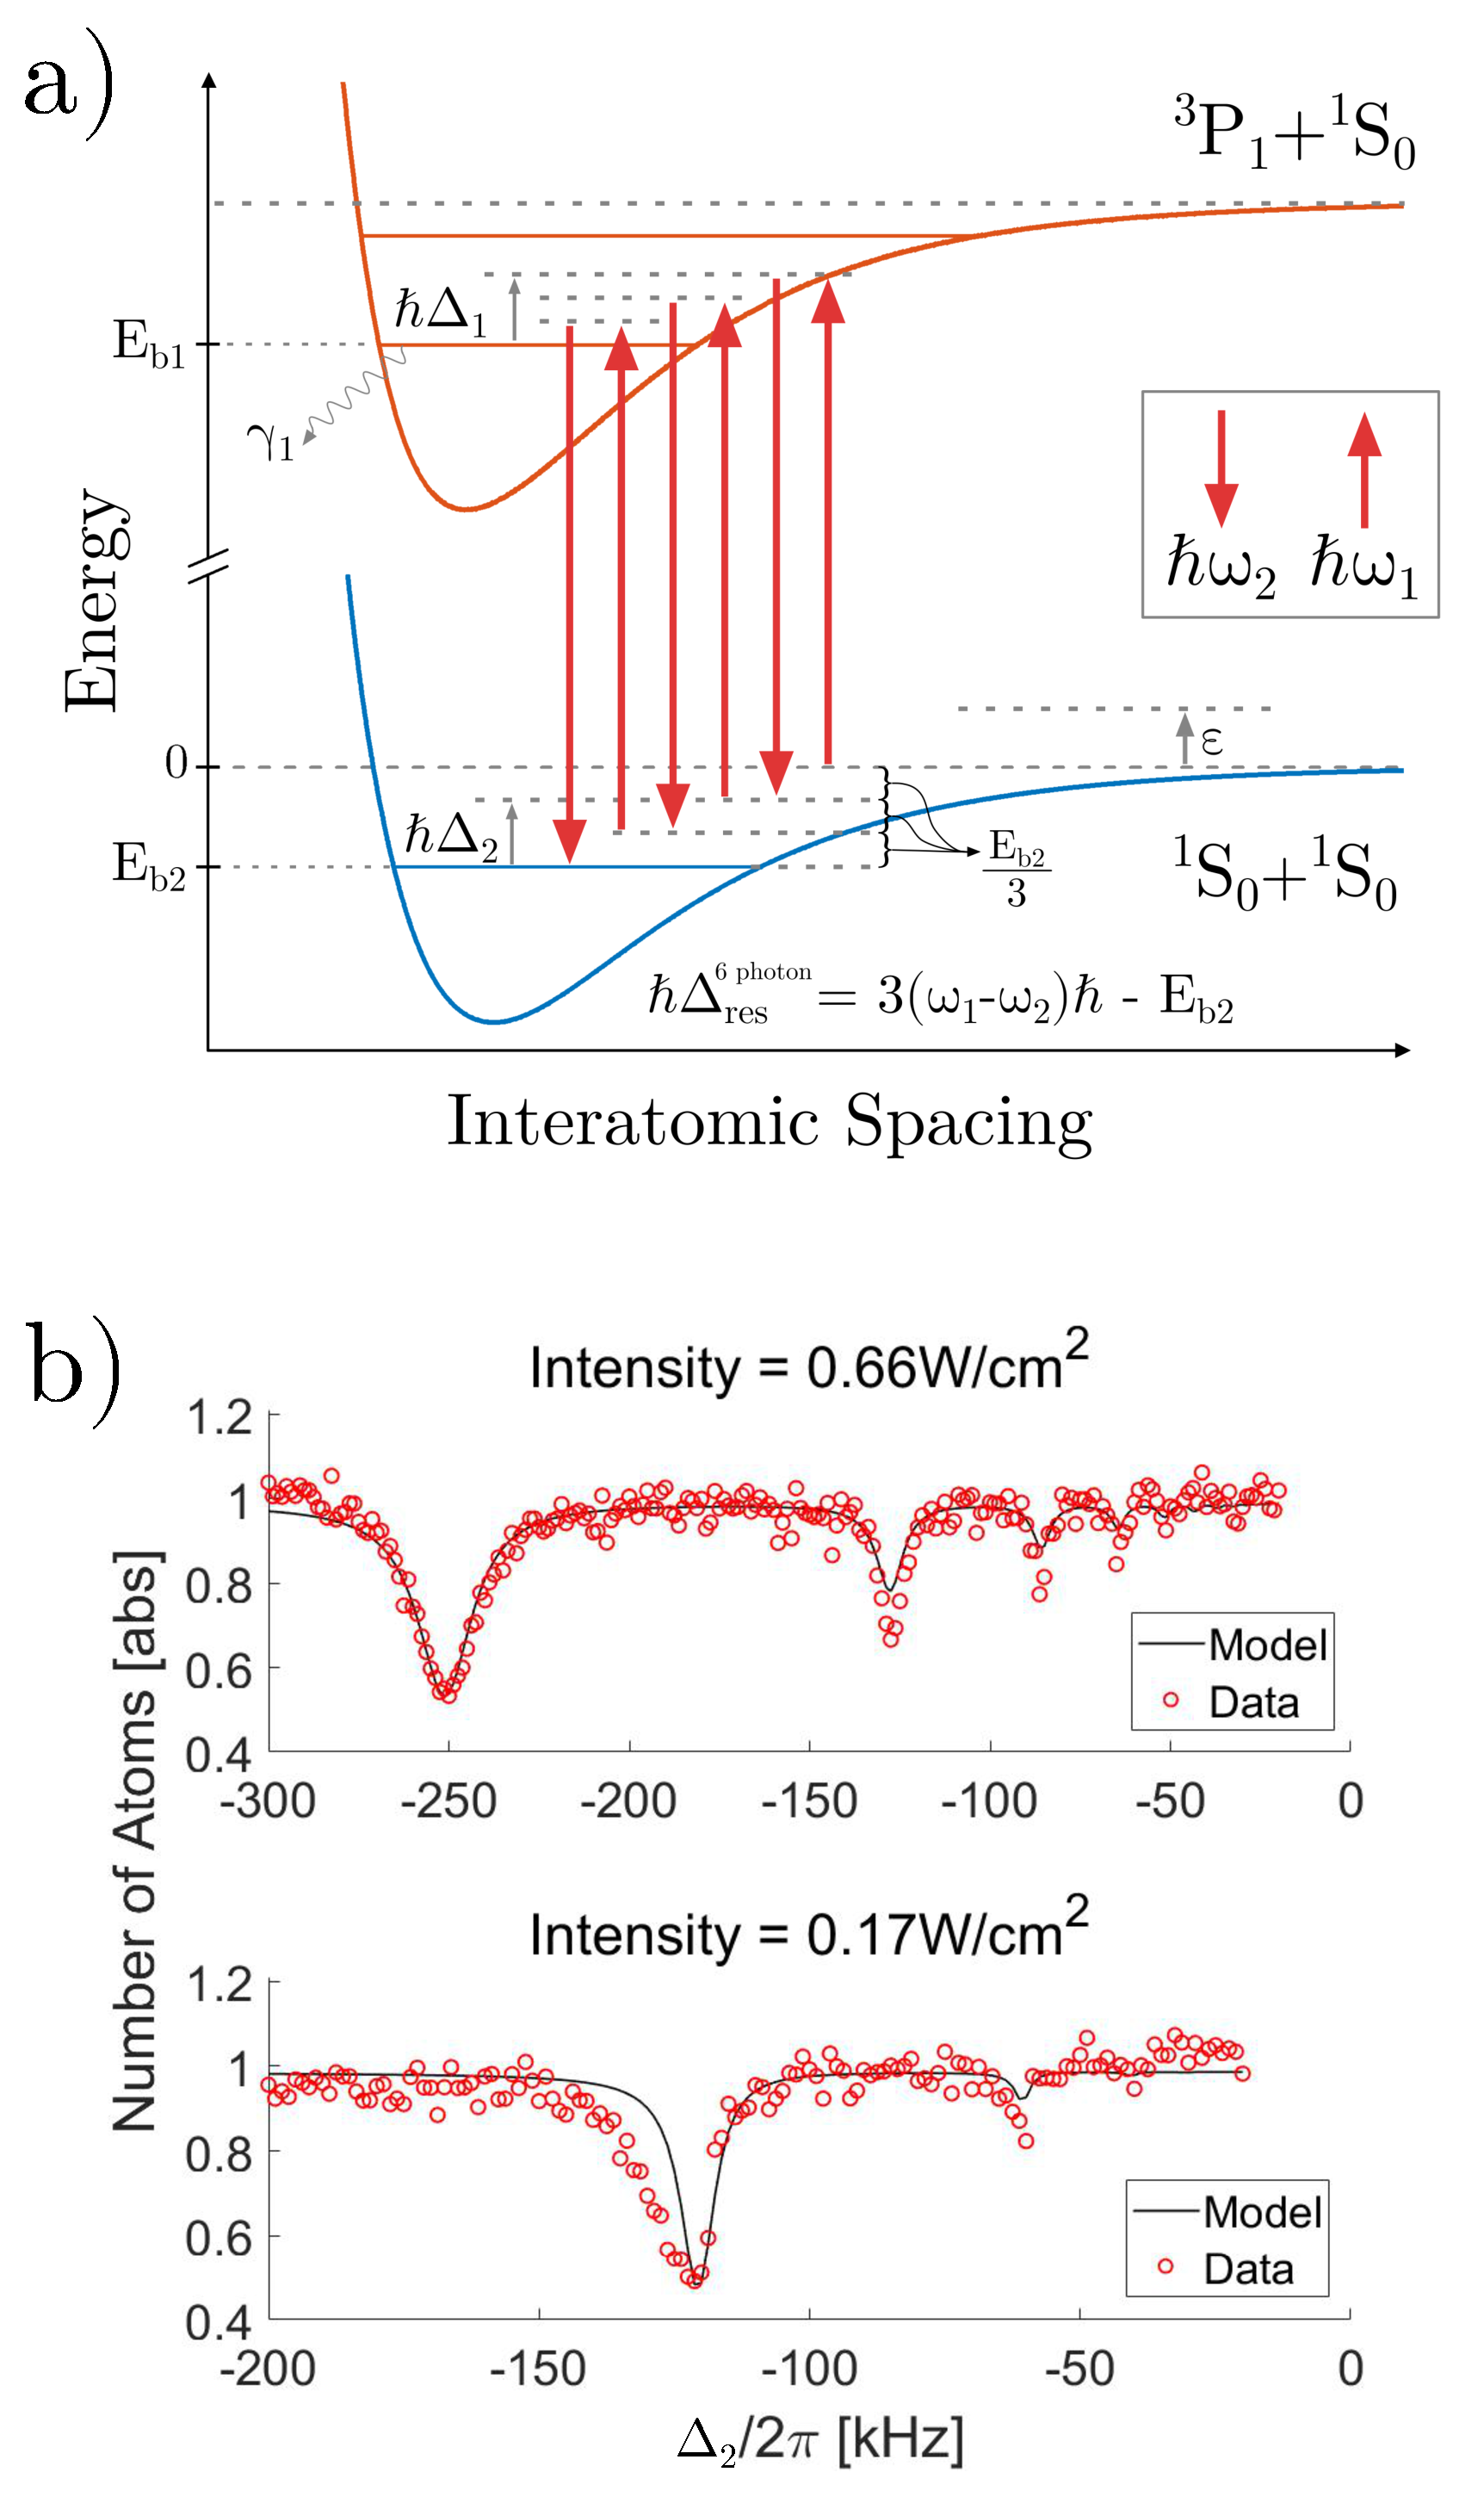
\includegraphics[width=\textwidth]{higherOrderModel.pdf}}
	  \caption{Multi-photon Raman processes}{a) The excitation process for observing multi-photon Raman processes. Shown is a 6-photon process which results in atom loss at $E_{b2}/3$ where $E_{b2}$ is the AC stark shifted halo molecule resonance energy of the fundamental process. b) Numerical simulation of the three-level model which reproduces the observed higher order loss processes.}
	  \label{fig:multiPhotonTheory}
	\end{figure}




%
%\begin{eqnarray} \label{equationSprob}
%  \vert S_{\epsilon 1}\vert^2 =   \hspace{2.5in}&&\\
%  {(\Delta_2+\epsilon/\hbar)^2{\gamma}_1{\gamma}_s \over
%  	\left[(\Delta_1+\epsilon/\hbar)(\Delta_2+\epsilon/\hbar)-\frac{\Omega_{12}^{2}}{4}\right]^2+\left[ \frac{\gamma_1+\gamma_s}{2}\right]^2(\Delta_2+		 	\epsilon/\hbar)^2}. &&\nonumber
%\end{eqnarray}
%
%
%describes a collision of two ground state atoms with total collision energy $\epsilon$, which leads to loss-producing decay from the excited state, $b_1$, with rate $\gamma_1$.
%
%Recall from our previous discussion that the form 
%For simplicity we use only the matri
%
% to neglect the additional loss channel due to loss from 
	
%In addition to the breakdown of the isolated-resonance model at high intensities and large detunings, we also observed novel loss features in the regime of strongest coupling between the halo state and the  as shown in 
%Such loss processes are not typically 	
%	
%For the highest intensity near measurements shown in Fig.\,\ref{fig:highIntMultiPhoton}
%These additional loss features are found to occur at intervals of 
%
%when the two laser are well separated
%
% we observe features absent in the lambda-model where only a single laser drives each leg of the PA process.
%Most notable are additional peaks near delw = pmEb/n for integer n, as shown in the spectra in Fig. 1(c-e).
%
% In Sec. VI, we will explain these peaks in terms of non-linear processes illustrated in Fig. 1(b) that become possible with the two-frequency drive.
%These additional peaks are more apparent at higher PA laser intensity and lower detuning
%
%
%Numerical simulations show that it accurately predicts the appearance of additional spectral lines in the high-intensity regime, and that these correspond to higher order non-linear processes.
%
%In this regime, additional peaks appear in the PA spectra at approximately Eb/2, Eb/3, . . ., as shown in Fig. 1(c). 
%This occurs at high intensities and/or low intermediatestate detunings, and we will refer to this as the “highintensity” regime throughout this paper. 
%We will discuss the origin of this effect in detail in Sec. VI. As per Fig. 1(c), we will refer to the most red-detuned line in the spectrum as the main negative peak, the most bluedetuned line as the main positive peak, and the additional peaks as higher order peaks.
	
	
	
	
%This demonstrates the origin of these higher order loss processes as a result of the small ovrall detuning $\Delta_2$ present in a simplified three-level scheme.
%Such higher order processes are therefore inherent in similar systems and not due to the excitation of the halo molecule.




%At high laser intensities and for relatively small single-photon detuning ($|\Delta_1|\lesssim 5$\,MHz), we observe additional spectroscopic features
%%that appear to be peculiar to Raman spectroscopy of a halo state. A
%as shown in Fig.\ \ref{Fig:multiphotondata}. For single-beam intensity $I$, the main feature appears at $\omega_1-\omega_2=E'_{b2}(I)/\hbar$, where $E'_{b2}(I)$ is shifted predominantly by the AC Stark shift from the excitation light, and
%additional features appear at
%subharmonics, $\omega_1-\omega_2=E'_{b2}(I)/n\hbar$ for $n=2,3..$ up to as high as $n=5$. The frequency pattern and the ratios of signal strengths suggest that the additional lines correspond to higher-order multi-photon Raman processes as shown in Fig.\ \ref{Fig:multiphotonschematic}, with the $n^{th}$ process involving $2n$ photons. A large negative AC Stark shift $\Delta_1<0$ %(Sec.\ \ref{sectionACStark})
%facilitates observation of this phenomena because it increases the binding energy of the halo state, stretching the frequency spectrum and making room for resolved subharmonics.
%
%In theoretical descriptions of photoassociation of colliding, ground-state atoms to weakly bound molecular levels on the ground-state potential, process of higher order than two-photon ($n=1$) were not considered \hl{\cite{bju96,bju99}}.
%To our knowledge, they have never been observed before now.
%%The similarity to a higher-order Bragg process might explain why this phenomena has not been seen before and highlights an unusual feature of photoassociation to a halo state.
%The extremely small binding energy associated with the halo state creates much more favorable conditions for observing this phenomena, however. It results in small intermediate detunings ($\sim E'_{b2}(I)/\hbar$), maintaining a high effective Rabi frequency for the multi-order process.
%
%There are similarities to other well-know spectroscopic phenomena. For example, non-linear Raman processes are commonly used in analytic chemistry, but  typically involves more, near-resonant laser fields \hl{\cite{bor82}} rather than just two as in our situation. Higher order Bragg spectroscopy of atoms, which can be viewed as a multi-order Raman process driven by two light fields, is perhaps more similar. This was developed in the context of atomic beams for atom interferometry \hl{\cite{dkc85,mom88,gml95}} and later applied to utlracold samples \hl{\cite{kdr96,kdh99,sic99}}. An important difference however, is that in Bragg spectroscopy, lasers are aligned for momentum transfer from the light fields to the atoms, making the resonance condition sensitive to initial atom momentum.
%
%
%
%To check whether our interpretation of higher-order processes is correct, we simulated the spectrum using a three-level lambda system connected by two coherent light fields, as shown in Fig.\ \ref{Fig:ThreelevelSystem}. This also
%will investigate whether the process depends on the fact that this is a scattering problem, involving an initial state of two free atoms.
%To model the loss, we assign loss rates of $\gamma_1=2\gamma_{atomic}$ to state $1$ and $\gamma_2=xx$,Hz to $2$ reflecting the broadening of the PAS line discussed in Sec.\ \ref{xx}. It is important to note that the Hamiltonian governing the system retains both laser fields in the coupling between states $0$ and $1$ and between $1$ and $2$. This is necessary because the frequencies of both laser fields are so similar, or, equivalently, the $0-2$ energy difference is so small. The $1-2$ coupling is set to the value determined from the observed AC Stark shift (Sec.\ \ref{sectionACStark}). The $0-1$ coupling is not well determined from the experiment, and it actually does not have a rigorous analog because the Hamiltonian doesn't reflect that state $0$ is a two-body scattering state. We simply use $\chi\ll 1$ as a fit parameter. Nonetheless, this simple approach captures the high-intensity spectrum extremely well.
%We find $\chi\ll 1$, showing the
%$1-2$ coupling is much stronger than the $0-1$ coupling, as observed in the experiment.
%

%%%%%%%%%%%%%%%%%%%%%%%%%%%%%%%%%%%%%%%%%%%%%%%%%%%%%%%%%%%%%%%%%%%%%%%%%%%%%%%%%%%%%%%%%%%%%%%%%
%%%%%%%%%%%%%%%%%%%%%%%%%%%%%%%%%%%%%%%%%%%%%%%%%%%%%%%%%%%%%%%%%%%%%%%%%%%%%%%%%%%%%%%%%%%%%%%%%

%Our model neglects motional effects. However, photoassociation is a scattering process, involving an initial state of two free atoms, and thus the collision amplitude will depend on energy

%The observed PA spectrum is relatively simple because the
%bosonic isotopes of strontium lack hyperfine structure. As shown in
%Fig.\ \ref{PASDiagram}, ground state $^1S_0$ atoms collide on a
%single $^1\Sigma^+_g$ potential. Four molecular potentials converge
%to the $^1S_0$ + $^3P_1$ asymptote \hl{\cite{mjs01}}, but only states of
%the $0^+_u$ and $1_u$ potentials are optically connected to the
%$^1\Sigma^+_g$ potential \hl{\cite{zbl06}}. At the low temperatures of
%these experiments, only $s$-wave collisions occur so only $J=1$
%intermediate levels and $J=0$ and 2 final states can be populated.


%The collision event rate constant can be expressed as a thermal average of the scattering probability for loss, $\vert S(\epsilon,\omega_1,\omega_2,...,\mathbf{r})\vert^2$, over the collision energy $\epsilon$. 

%We also average over the trap volume to allow for the possibility that the scattering probability can vary with position in the trap due to inhomogeneity of laser intensity profiles and the density distribution [Eq.~(\ref{equationKeffective})].

%Bohn and Julienne \hl{\cite{bju96}} provide an expression for $\vert S(\epsilon,\omega_1,\omega_2,...)\vert^2$ for a collision on the open channel of two ground state atoms (g) with total energy $\epsilon$ leading to loss-producing decay from the excited state $b_1$ with rate $\gamma_1$. (See Fig.\ \ref{PASDiagram}.) It yields
%\begin{eqnarray}\label{equationSprob}
%  \vert S\vert^2 =   \hspace{2.5in}&&\\
%  {(\Delta_2+\epsilon/\hbar)^2{\gamma}_1{\gamma}_s \over
%  	\left[(\Delta_1+\epsilon/\hbar)(\Delta_2+\epsilon/\hbar)-\frac{\Omega_{12}^{2}}{4}\right]^2+\left[ \frac{\gamma_1+\gamma_s}{2}\right]^2(\Delta_2+		 	\epsilon/\hbar)^2}, &&\nonumber
%\end{eqnarray}
%where all quantities are defined in the main text. For simplicity, we have omitted the light shift of $b_1$ due to coupling to the scattering continuum \hl{\cite{bju99}}. Equation (\ref{equationSprob}) neglects all light shifts due to the trapping laser. Light shifts due to the photoassociation lasers coupling to states outside our model (Fig.\ \ref{PASDiagram}) are also neglected. The thermal energy is much greater than the zero-point energy for trap motion, $T\gg h\nu_{\text{trap}}/k_B$, so confinement effects are negligible \hl{\cite{zbl06}}.

%For the experiments reported here, we maintain significant intermediate-state detuning, $|\Delta_1|\gg |\Omega_{12}|$. Thus we are in a Raman configuration, and near two-photon resonance the expression for the scattering probability for a given initial scattering energy Eq.~(\ref{equationSprob}) can be approximated as a Lorentzian
%\begin{eqnarray}\label{equationSprobLorentzian}
% \vert S\vert^2 \approx {A(\epsilon) \over
% \left(\Delta_2+\epsilon/\hbar-\frac{\Omega_{12}^{2}}{4(\Delta_1+\epsilon/\hbar)}\right)^2+\left[ {\Gamma_L(\epsilon)}/{2}\right]^2},
%\end{eqnarray}
%where $A$ and $\Gamma_L$ are defined in Eqs.\ (\ref{ApproxLorentzianQuantitiesMain}) and (\ref{ApproxLorentzianQuantities-2Main}).
%
%As discussed in the text, we analyze loss spectra using the effective expression, Eq.\ (\ref{equationApproxLorentzian}) to account for possible deviations from the single-channel theory \hl{\cite{bju96}}.

%follows $\delta={\Omega_{12}^{2}}/{2\Delta_{1}}$ in agreement with Eq. \ref{Eq:ACStarkFullModel}.
%If  a  single-resonance model, only describing coupling of the halo state $b_2$ to the intermediate state $b_1$, were accurate, then
%\begin{equation}\label{Eq:ACStarkFullModel}
%\chi_{689}\equiv \frac{\Omega_{2,12}^{2}}{8\pi\Delta_{1}}+\frac{\Omega_{1,12}^{2}}{8\pi\left(\Delta_{1}-E_{b2}\right)}
%\end{equation}
%We model the Stark shift  with a single resonance model,
%\begin{equation}\label{Eq:ACStarkFullModel}
% E'_{b2}\equiv E_{b2}+\frac{\hbar\Omega_{2,12}^{2}}{4\Delta_{1}}+\frac{\hbar\Omega_{1,12}^{2}}{4\left(\Delta_{1}-E_{b2}\right)}=
% E_{b2}+h\chi_{689}(\Delta_{1}) I_{689},
%\end{equation}
%where we have separated the contributions from the two beams, but for all data discussed here, both intensities are equal and $\Omega_{2,12}=\Omega_{1,12}$. The small difference in detunings of the two beams is shown but produces a negligible effect.

%It is important to note that the total 689-nm intensity oscillates with 100\% contrast according to
%$I_{total}=I_1+I_2+2\sqrt{I_1I_2}\cos \left[(\omega_1-\omega_2)t \right]=2I\left\{1+\cos \left[(\omega_1-\omega_2)t \right]\right\}$.
%Equation \ref{Eq:ACStarkFullModel} assumes assumes the AC Stark shift reflects the time average of the intensity and neglects the interference term. To confirm that this is the correct description, we numerically solved the time-evolution for a three-level system. The Hamiltonian is
%\begin{eqnarray}\label{Eq:ThreeLevelHamiltonian}
%H= \hspace{3in} \\
%\left(
%    \begin{array}{ccc}
%      0 & \Omega_{01}\left[\mathrm{cos}(\omega_1 t)+ \mathrm{cos}(\omega_2 t)\right] & 0 \\
%      . & E_{b1} & \Omega_{12}\left[\mathrm{cos}(\omega_1 t)+ \mathrm{cos}(\omega_2 t)\right] \\
%      . & . & E_{b2} \\
%    \end{array}
%  \right)
%\nonumber
%\end{eqnarray}
%For  $\Omega_{01}\ll \Omega_{12} \ll \Delta_{1}\equiv E_{b1}/\hbar-\omega_1$, which is analogous to the  coupling scheme for photoassociation, the shift of the two-photon resonance condition follows $\delta={\Omega_{12}^{2}}/{2\Delta_{1}}$ in agreement with Eq. \ref{Eq:ACStarkFullModel}.


%(What is the AC Stark shift form the atomic transition on a single atom? The sign of the contribution from the unidentified state suggest that this is the main contribution as the red light approaches atomic resonances.
%
%Add in the figure just the contribution of the 1S0-3P1 atomic transition to the shift of the colliding atoms (2 x the single atom shift).)


%\begin{equation}\label{Eq:ACStarkFullModel}
% E'_{b2}\equiv E_{b2}+\frac{2\Omega_{12}^{2}}{4\Delta_{\nu=-2}}+
% \frac{2\Omega^{'2}}{4\Delta_{\nu=-1}},
%\end{equation}
%where $\Omega_{\alpha,b2}$ is the Rabi frequency for coupling between the halo state and state $\alpha$ of the $0^+_u$ molecular potential, and $\Delta_{\alpha}$ is the detuning of the 689 nm laser from resonance with the single-photon photoassociative transition to state $\alpha$.
%The factor of two before each Rabi frequency reflects %the fact that both excitation lasers contribute to the Stark shift with roughly equal detuning.


%}
%comment on loss for a given change...perhaps show large shift-data.

%\section{Higher-Order Raman Processes
%\label{sectionMultiphoton}}
%
%%For atoms, directed in the context of atom interferometry, as a coherent atomic beam splitter. First observation of Bragg scattering of atoms in a beam from a standing wave of light, including higher-order processes (up to 4th order - 9 photons mentioned) \hl{\cite{mom88}}.(Absorption and stimulted emission of photons. Energy and momentum are conserved. Resonantly tuned so that atoms scatter mainly into one order. Kapitza-Dirac scattering had been observed previously.) Standing wave was fixed. Atoms came in with finite momentum that satisfied the Bragg condition for $\Delta E=0$.
%%
%%Careful study in similar experiments, observed up to 6th order \hl{\cite{gml95}}.
%%Proposed in JETP paper \hl{\cite{dkc85}}.
%%
%%With advent of essentially stationary atoms.increased control..Bragg spectroscopy from a moving standing wave starting with atoms in a BEC \hl{\cite{kdh99}}
%

